% !TEX TS-program = xelatex
% !TEX encoding = UTF-8
% V8 research manuscript, rebuilt from the user's original aas project.
\RequirePackage{iftex}
\ifXeTeX\else\PackageError{UAV-GSL-V8}{Use XeLaTeX}{Select XeLaTeX in Overleaf.}\fi
\PassOptionsToPackage{fontset=fandol}{ctex}
\documentclass{aas}
\usepackage{amsmath,amssymb,bm,mathtools}
\usepackage{graphicx,booktabs,tabularx,array,multirow}
\usepackage{ccaption,microtype,placeins,xcolor,enumitem}
\usepackage{tikz}
\usetikzlibrary{arrows.meta,positioning,calc,fit,shapes.geometric}
\usepackage{xurl}
\usepackage[unicode,hidelinks]{hyperref}
% Portable fonts included with standard TeX Live / Overleaf; no system-specific paths.
\IfFontExistsTF{TeX Gyre Termes}{\setmainfont{TeX Gyre Termes}}{\setmainfont{Latin Modern Roman}}
\IfFontExistsTF{TeX Gyre Heros}{\setsansfont{TeX Gyre Heros}}{\setsansfont{Latin Modern Sans}}
\setCJKmainfont{FandolSong-Regular.otf}[BoldFont=FandolSong-Bold.otf,ItalicFont=FandolKai-Regular.otf]
\setCJKsansfont{FandolHei-Regular.otf}[BoldFont=FandolHei-Bold.otf]
\setCJKmonofont{FandolFang-Regular.otf}
% Small OFL-licensed renamed subset for the verified author character 鋆.
\IfFileExists{fonts/V8ReferenceFallback.otf}{%
  \setCJKfallbackfamilyfont{\CJKrmdefault}[Path=fonts/]{V8ReferenceFallback.otf}%
}{\IfFileExists{../fonts/V8ReferenceFallback.otf}{%
  \setCJKfallbackfamilyfont{\CJKrmdefault}[Path=../fonts/]{V8ReferenceFallback.otf}%
}{}}
\xeCJKsetup{PunctStyle=quanjiao,AutoFallBack=true}

\hypersetup{pdftitle={双侧镜像嗅觉与主动反证驱动的无人机气体源概率定位},pdfauthor={},pdfsubject={V8研究稿，非投稿定稿},pdfkeywords={气体源定位，镜像嗅觉，源判别，主动感知}}
\setlength{\abovedisplayskip}{6pt plus 2pt minus 2pt}
\setlength{\belowdisplayskip}{6pt plus 2pt minus 2pt}
\setlength{\jot}{3pt}
\setlength{\parindent}{2em}
\setlength{\parskip}{0pt}
\setlength{\emergencystretch}{2em}
\setlist{nosep,leftmargin=1.7em,topsep=3pt}
\newcommand{\I}{\mathbb{I}}
\newcommand{\R}{\mathbb{R}}
\newcommand{\E}{\mathbb{E}}
\newcommand{\KL}{\operatorname{KL}}
\newcommand{\JS}{\operatorname{JS}}
\newcommand{\ccite}[1]{\nobreak\cite{#1}}
\newcommand{\pending}{\textit{待执行}}
\newcommand{\researchstatus}[1]{\par\noindent\textbf{验证状态.} #1\par}
\newcolumntype{Y}{>{\raggedright\arraybackslash}X}
\renewcommand{\refname}{\centering\normalsize\bfseries 参考文献}
% Remove fake journal volume, issue, author and DOI fields in this research draft.
\makeatletter
\AtBeginDocument{%
\def\ps@aas@firstheadings{\let\@oddfoot\@empty\let\@evenfoot\@empty
 \def\@oddhead{\vbox{\hbox to\textwidth{\small 无人机气体源概率定位研究稿\hfill V8\quad 2026-10-23\quad\thepage}\vskip2mm\hrule}}\let\@evenhead\@oddhead}
\def\ps@aasheadings{\let\@oddfoot\@empty\let\@evenfoot\@empty
 \def\@oddhead{\vbox{\hbox to\textwidth{\small 双侧镜像嗅觉与主动反证定位\hfill V8 研究稿\quad\thepage}\vskip2mm\hrule}}\let\@evenhead\@oddhead}
}
\makeatother
\begin{document}
\cntitle{双侧镜像嗅觉与主动反证驱动的\\无人机气体源概率定位}
\cnauthor{研究讨论稿}
\cnabstract{针对间歇羽流下有限局部测量难以区分竞争气源、错误源判断可能持续影响后续采样的问题，研究以同步双机嗅觉观测为输入的气体源概率定位方法。构建源判别导向的双侧镜像嗅觉联合通道，将因果时间滤波、非线性整流和左右镜像相减用于提取候选源相关差异，并在同一观测块内联合建模共模强度与镜像响应；利用动态气味边界的进入方向记忆约束候选测量区域，以源响应差选择双机基线；在完整合法源集中进行成本约束的反证动作分配，以新观测后缀审计当前源判断。主输出为二维源位置概率图，审计结果仅影响后续决策。基于已恢复的8个原生GADEN归档世界，在两个已标定源、4个独立开发世界的粗采样理想浓度读出对照中，普通单点及完整双点方法均为4/4严格判对，当前镜像通道选择方法为2/4，平均平面MAP误差2.427\,m。训练目标提前饱和导致动态镜像通道未被选入，尚未建立相对普通联合观测的独立增益。本文据此给出完整方法研究稿、条件性理论及分层验证方案，双机主动闭环和湖岸泛化性能仍待检验。}
\cnkeyword{气体源定位，双侧镜像嗅觉，竞争源判别，主动感知，序贯假设检验，源概率图}
\entitle{Probabilistic UAV Gas Source Localization via Bilateral Opponent Olfaction and Active Falsification}
\enauthor{Research manuscript}
\enabstract{Intermittent plumes can make competing gas sources difficult to distinguish from limited local measurements, while an incorrect source belief can influence subsequent sensing. This manuscript develops a probabilistic localization method using synchronized observations from a pair of UAVs. A source-discriminative bilateral opponent channel combines causal temporal filtering, rectification, and mirrored subtraction, and jointly models common intensity and opponent responses within each observation block. Entry-direction memory at dynamic odor boundaries proposes sensing regions, while differences between source-conditioned responses determine the sensing baseline. Cost-constrained action allocation retains all admissible sources and uses a fresh observation suffix to audit current source hypotheses. The primary output is a two-dimensional source probability map; audit statistics affect future decisions without being counted again as gas evidence. A bounded comparison used eight restored native GADEN archive worlds, with two calibrated source locations and four independent development worlds under coarse sampling and ideal concentration readout. Ordinary single-point and full paired-observation methods classified all four development worlds correctly, whereas the current channel-selection method classified two, with a mean planar MAP error of 2.427 m. Its training objective saturated before any dynamic opponent channel was selected. The present evidence therefore does not establish a localization advantage. The manuscript specifies the algorithms, conditional theoretical statements, and controlled validation plan; native dual-UAV closed-loop performance and lakeshore generalization remain to be tested.}
\enkeyword{gas source localization, bilateral opponent olfaction, source discrimination, active sensing, sequential hypothesis testing, source probability map}
\makeatletter\gdef\aas@doi{}\gdef\caddress{}\gdef\aas@enaddress{}\makeatother
\maketitle
\pagestyle{aasheadings}
\raggedbottom
\section{引言}
危险气体泄漏的应急处置需要尽快确定泄漏位置，为人员避险、设备检修与后续监测提供依据。携带气体传感器的无人机能够进入岸坡、设施间隙等不便接近的区域，但其可获得的通常只是飞行轨迹上的局部浓度、风和位姿。气体源定位因此是由有限受体观测推断未知释放位置的逆问题；气体分布建图回答的则是气体在空间中如何分布，两者可以相互支持，却具有不同的估计对象与评价指标\ccite{Francis2022,Gongora2023}。

气体传播的随机性与传感器的有限响应共同限制了这种反演。同一固定源可在不同传播实现中产生不同的到达时刻和间歇片段，不同源也可能在已有测点上形成近似响应。湖岸地形与水陆边界进一步使局地风和气体实际经历的传播条件存在差别，相关微气象研究揭示了湖风锋及跨岸浓度梯度的时空变化\ccite{Welch2024,Huang2024}。无人机旋翼、传感器布置及平台间干扰还会影响气体读出\ccite{Ercolani2023}。因此，局部浓度峰值、重捕获羽流和源位置确认之间不能直接画等号。

现有研究主要通过行为搜索、源条件模型反演及信息驱动采样应对上述困难。行为搜索根据气味事件、梯度与风向调整运动；双侧浓度和动物趋性已被用于三维气味源定位\ccite{Lin2025Bilateral}，近期昆虫启发的感知补偿方法也在机器人上研究了嗅觉缺损下的搜索行为\ccite{Shigaki2026Adaptive}。这些成果说明双侧感知、记忆或气味重捕获本身已有先例，新的定位方法需要进一步说明其如何区分具体竞争源。源条件模型通过预测不同释放位置的响应，将局部观测转化为位置证据。地形感知学习与数据驱动羽流模型分别从环境结构和观测数据出发研究定位与传播表达\ccite{Tian2025,Jin2023}；概率建图与前向仿真方法（probabilistic mapping and forward simulation, PMFS）则利用观测命中图、候选源在线传播和带置信度的地图比较，持续输出源位置分布\ccite{Ojeda2024PMFS}。近期预印本中的物理依赖顺序推断也直接研究了连续浓度、风和源之间的概率关系\ccite{Kim2026DGSE}；因此，源导向建模本身不是本文独有的研究方向。

主动采样进一步决定机器人能够获得哪些证据。信息趋向搜索以预期信息量驱动探索\ccite{Vergassola2007Infotaxis}，运动中感知、置信聚类与累积信息路径规划将观测与运动过程更紧密地结合\ccite{Jin2024,Jin2025}。PMFS 本身也根据候选源预测差异与未观测区域置信度选择下一测点，并非被动处理固定航线数据\ccite{Ojeda2024PMFS}。这些方法已经建立了概率推断和主动搜索的基本链条，仍需进一步考察：候选源预测的分歧是否能够在实际传感器带宽和驻留时间下被读出，以及错误后验是否会使后续观测持续偏向同一错误解释。

上述问题具有明确的源级检验对象。提高完整浓度场的预测精度，不一定改善竞争源之间的似然比；压缩后的空间命中统计，也未必保留双点观测的所有时空关系。另一方面，增加第二架无人机只增加了测量资源，不能自动证明新的算法贡献。已有项目中的错误高置信、预测误差下降但源排序未改善、多个候选仍与有限观测相容等记录，提示应同时研究判别表示、测量几何与持续反证；这些记录的条件不同，并未建立统一失效根因，具体证据见第\ref{sec:motivation}节。

双侧嗅觉神经计算为构造可解释的时间表示提供了一条具体途径。Brudner 等提出由双侧时间滤波、非线性整流和镜像相减组成的模型，用于解释果蝇在不同羽流中的梯度与气味运动线索利用\ccite{Brudner2026Opponent}；其原始目标是羽流中心线侧别与转向行为，而非未知释放点的概率定位。Siliciano 等研究了以气味进入方向为记忆的动态边界导航策略\ccite{Siliciano2026Vector}。将这些机制用于气源定位，需要将行为目标转成可检验的源条件观测差异，并与实际运动成本和错误源假设复核相连接。主动序贯多假设检验与可预测似然审计为后一个环节提供了数学基础\ccite{Hsu2025Tradeoffs,Vershinin2026Costs,Wasserman2020Universal,Zecchin2025QSUT}。

基于此，本文围绕有限采样条件下的竞争源辨识，形成双侧镜像嗅觉、判别式双机测量和主动反证相衔接的方法研究稿。两架无人机作为一组同步嗅觉观测平台，主输出保持为二维源位置概率图。三个方法贡献的设计分别如下。

\textbf{1) 源判别导向的双侧镜像嗅觉联合通道。}将母方法的方向判别算子转化为源条件观测表示，在有限合法滤波核库中按竞争源对分离选择通道，并将共模强度与镜像差异编码为一个联合符号。新增设计集中于源对目标、联合标定和一次证据更新；镜像滤波本身及贝叶斯归一化不作为原创。当前实现采用固定核库选择，其原生开发对照已暴露覆盖目标提前饱和的问题。

\textbf{2) 动态边界记忆约束的判别式双机测量。}将实际气味进入方向用于提出候选测量区域，再根据训练响应的均值差、梯度差与协方差选择双机间距和方向。当记忆区域不足以区分源时，保留返回记忆区域外、物理合法域内的付费复测，使边界重捕获服务于源辨识。该设计的独立收益需在相同双机资源与原始观测权限下验证。

\textbf{3) 完整候选源的成本约束反证与恢复。}对全部合法竞争源构造动作条件分离量，在实际移动与驻留成本下分配观测，并混合不依赖源后验的覆盖动作；以新观测后缀对当前源假设进行审计，允许当前相容列表恢复。审计统计量只影响后续采样，不作为独立气体证据再次乘入源后验。风险控制的结论以真实过程属于正确条件观测族为前提。

本文已经完成方法接口与有界原生开发对照的整理，尚未建立三个模块的独立定位增益。第2节给出任务与研究动机，第3、4节说明实际算法和条件性结论，第5节如实报告已有结果并规定后续验证，第6节总结当前认识及适用边界。

\section{问题描述与研究动机}
\subsection{场景、观测任务与固有挑战}
\label{sec:task}
图\ref{fig:scene}给出湖岸设施附近的目标应用场景。未知固定源位于物理允许的释放区域，气体在地形、障碍和局地风作用下传播。两架无人机组成同步测量单元，获取气体序列、采样位置与局地测风，并根据已有观测更新源位置判断和下一测量动作。背景图中的两机及轨迹用于说明测量任务，不是枫树岭S2的已验收浓度场。本文的单源任务与后续多机任务分配研究分开。

\begin{figure*}[t]
\centering
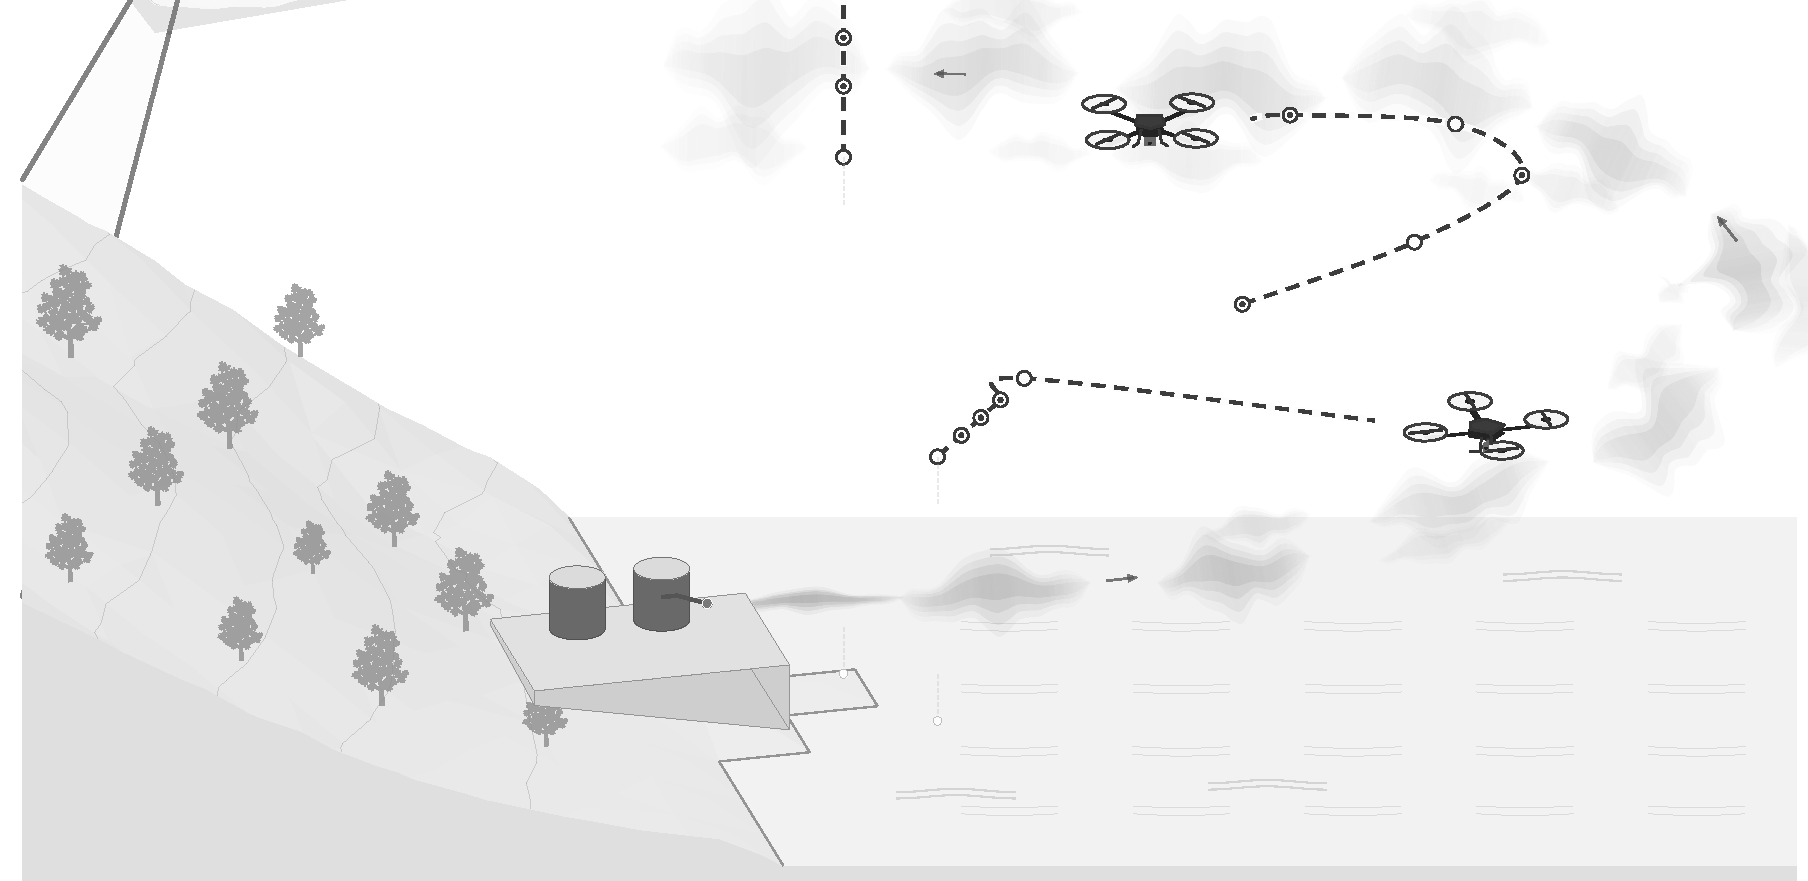
\includegraphics[width=0.97\textwidth]{figures/fig1_scene.pdf}
\caption{湖岸气体源定位目标应用场景。复用原可编辑研究背景图；双机同步测量的几何定义见图\ref{fig:geometry}。该图为概念示意，源概率图是本文主输出，未将场景图解释为已完成的湖陆风或三维羽流验证。}
\label{fig:scene}
\end{figure*}

记物理源可存在域为$\Omega_{\rm src}$，飞行可达域为$\Omega_{\rm fly}$，传感器有效采样域为$\Omega_{\rm obs}$。三者分别由释放条件、飞行安全及传感器安装位置确定，不能以二维导航自由格替代全部合法源。候选源集合为$\mathcal S=\{s_j\}_{j=1}^J\subset\Omega_{\rm src}$，$s_j=(x_j,y_j,z_j)^{\mathsf T}$，真实固定源为$s^*$。有限候选集合内的分类性能与连续未知源的定位精度分别评价。

以$t$表示决策或观测块编号，以$\tau_{t,n}$表示第$t$块中第$n$个样本的物理时间。左右传感器标记为$u\in\{L,R\}$，实际采样位置为$\mathbf x^u_{t,n}\in\R^3$，气体读数为$y^u_{t,n}$，局地测风为$\widehat{\mathbf v}^u_{t,n}$。原始同步观测块写为
\begin{equation}
 X_t=\big\{\tau_{t,n},\mathbf x^u_{t,n},y^u_{t,n},
 \widehat{\mathbf v}^u_{t,n}\big\}_{n=1,u\in\{L,R\}}^{N_t}.
 \label{eq:block}
\end{equation}
世界坐标、测点外参、两侧时钟及浓度单位需在形成$X_t$之前统一；不可用相邻世界、未来风或事后平移的真源历史拼成同步块。局地风仅在实际可用时进入算法，缺测和不具备竖直风分量必须保留标记。

给定源、传播状态及传感器参数，读数可统一表示为
\begin{equation}
 y^u_{t,n}=\mathcal G_{\psi_u}\!\left[
 C\!\left(\mathbf x^u(\tau),\tau;s_j,\eta\right),m^-_{u,t}
 \right](\tau_{t,n})+\varepsilon^u_{t,n}.
 \label{eq:sensor}
\end{equation}
其中$C$为三维物理浓度，$\eta$包括未知释放强度、传播条件等干扰量，$\mathcal G_{\psi_u}$表示经校准的传感器动态，$m^-_{u,t}$为该块开始前的实际响应状态，$\varepsilon^u_{t,n}$为测量噪声。原生GADEN及GADEN-RT为候选传播和受体浓度提供仿真工具\ccite{Monroy2017GADEN,Ojeda2025GadenRT}，但仿真浓度与真实PID读数不能不经说明地等同。第5节的归档实验使用理想零延迟浓度查询，不检验式\eqref{eq:sensor}中的真实传感器动态。

地图和障碍为$G$，冻结训练资料及事前配置为$\mathcal D_{\rm tr}$。本稿以$X_t$表示用于M1的同步采样窗；截至第$t$步结束已经取得的行进期气体、位置、运动方向及可用局地风另记为$H_t^{\rm tr}$。完整已发生历史定义为$\mathcal F_t=\sigma(G,\mathcal D_{\rm tr},X_{1:t},H_t^{\rm tr},a_{1:t})$，因此行进期数据虽不进入当前驻留块似然，也属于策略实际可见的信息。动作$a_t$包含两机实际路径、测量中心、基线长度与方向、采样高度及驻留时间，基于$\mathcal F_{t-1}$及与环境独立的控制随机数选定，并在新观测出现前固定。任务资源由移动、停留、传感器数量和计算成本共同约束。定位主输出为源质量$\pi_t(s_j)$及其二维投影
\begin{equation}
 P_t(g)=\sum_{j:\Pi(s_j)\in g}\pi_t(s_j),\qquad
 \sum_g P_t(g)=1,
 \label{eq:projection}
\end{equation}
其中$\Pi(s_j)=(x_j,y_j)$，$g$为二维源图单元。候选源高度未知时应将合法高度作为候选或共享机制建模，再按式\eqref{eq:projection}边缘化；不能删除不在导航平面的源后仍声称覆盖其物理位置。输出同时保留MAP集合、概率覆盖情况及当前审计列表，后者不等同于概率图。

这一任务具有三方面固有困难。其一，间歇传播与未知风历史使相同源的有限窗响应变化，不同源也可能产生近似观测。其二，有限测点与有限带宽限制可观测尺度，两侧延迟不一致甚至可产生并不存在的运动线索。其三，飞行几何、源位置支持和受体体积处于不同尺度，空间合法性不能由单一地图替代。这些困难独立于所采用的定位算法；高保真三维预测、额外测量平台或更长历史是否有用，最终都需由源判别结果说明。

\subsection{原生PMFS计算链及具体研究动机}
\label{sec:motivation}
PMFS利用局地浓度与风构造空间气体命中概率和采样置信度，通过候选源的简化二维丝团传播预测命中图，再按地图兼容程度得到源位置分布。其主动选点利用源分布加权的候选响应方差与未观测置信度\ccite{Ojeda2024PMFS}。图\ref{fig:pmfs}复用V7中对原方法的可编辑示意。这里将论文原理与具体代码版本分开：实现审计固定于作者仓库提交\texttt{4e141e1}，项目O24的作者代码来源固定于\texttt{a8d5a76}，未将前一版本的实现细节当作后一版本的实跑结论\ccite{V7Archive}。

\begin{figure*}[t]
\centering
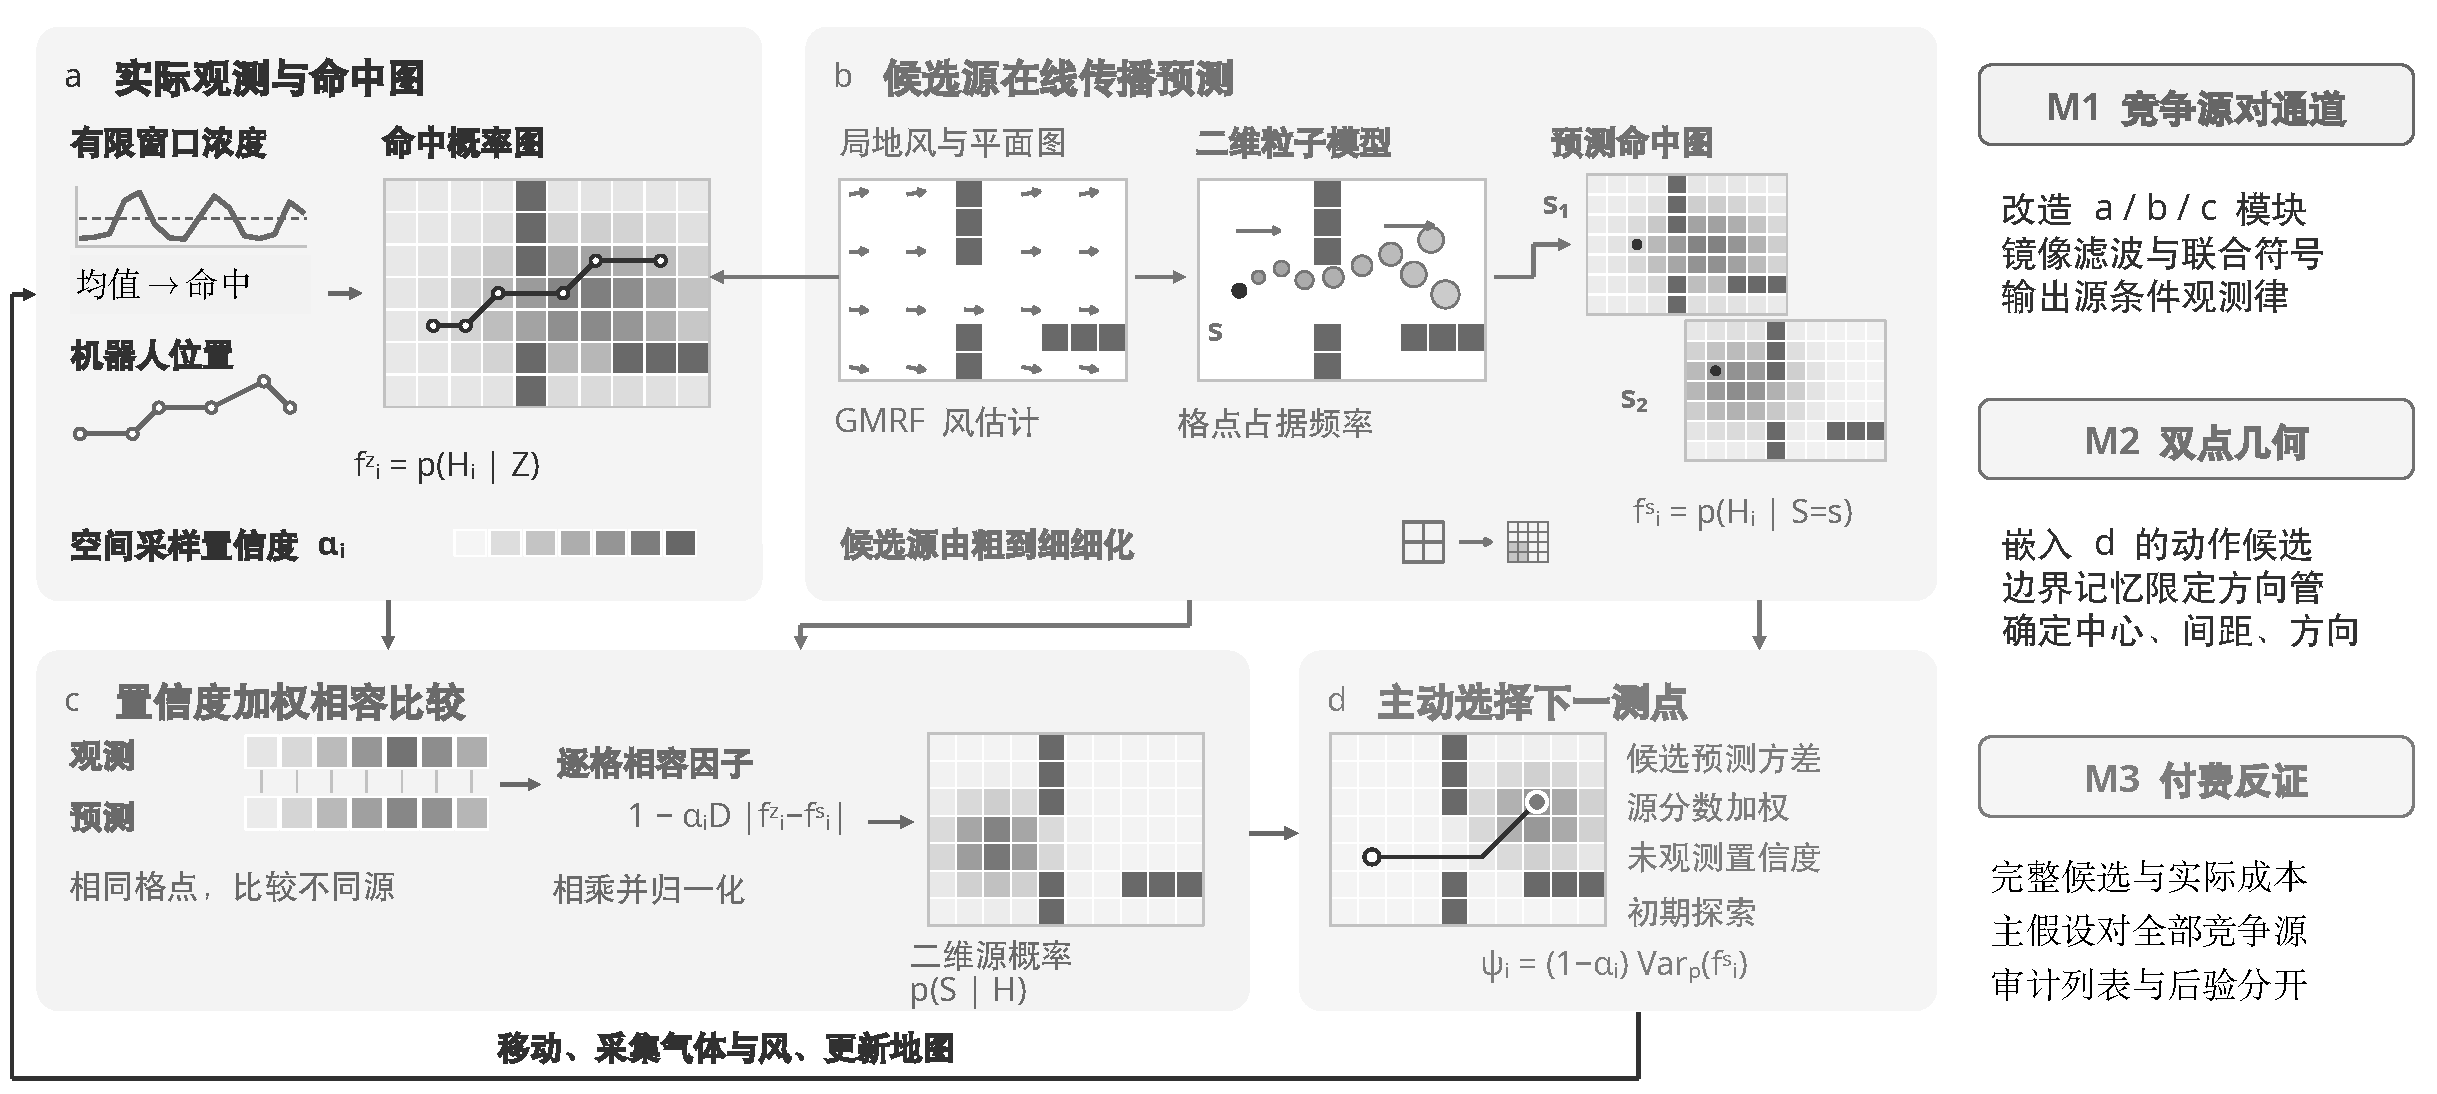
\includegraphics[width=0.98\textwidth]{figures/fig2_pmfs.pdf}
\caption{原生PMFS的观测命中图、候选传播、兼容评分和主动选点，以及本文对应的观测表示与决策接口。图源为V7可编辑方法图第1页；正文区分论文原理和固定代码版本。二维命中图与二维源概率图具有不同含义。}
\label{fig:pmfs}
\end{figure*}

上述被审计实现对有限停留窗内的平均浓度阈值化，再以风相关空间核传播命中事件并累积地图信息。令$p_{i,t}$为第$i$格当前观测命中概率，$h_{i,t}(s_j)$为候选预测频率，$c_{i,t}$为采样置信度，$D$为固定兼容系数，则源评分的实际结构为
\begin{equation}
 \widetilde\pi^{\rm PMFS}_t(s_j)=
 \prod_{i\in\mathcal V_{\rm free}}
 \bigl[1-c_{i,t}D\lvert p_{i,t}-h_{i,t}(s_j)\rvert\bigr].
 \label{eq:pmfscompat}
\end{equation}
归一化后的评分覆写源图，历史主要通过累计命中图进入。式\eqref{eq:pmfscompat}不额外乘前次源后验，因此不能将其错误描述成每轮重复乘入旧后验。相同局地事件可影响多个地图单元，这些单元间的依赖及观测/预测读出定义是否匹配，才是需要控制实验检验的问题。该版本实际选点所用的主要代理量为
\begin{equation}
 V_t(x)=\bigl[1-c_t(x)\bigr]
 \operatorname{Var}_{\pi^{\rm PMFS}_t}
 \{h_t(x;S)\}.
 \label{eq:pmfsplanning}
\end{equation}
它体现候选预测分歧，但不是已校准的有限驻留传感器互信息。测量噪声、带宽和候选分布形状均可能改变实际可分性，不能仅凭均值方差较大推断单位时间的源信息较多。

表\ref{tab:motivation}将研究动机限定在已有证据能够支持的层次。B4错误高置信是停止条件与真实位置准确性不一致的实例；M4/RK对照说明预测损失与定位目标不等价；有限观测相容性记录说明少量观测可能不足以排除多个源。各例的数据权限、源支持、观测窗口和模型不同，不能合并成一个已经确认的物理根因。

\begin{table*}[t]
\centering\small
\caption{动机证据、允许推论及其限制。历史诊断与V7开发对照不是同一数据集上的方法排名。}
\label{tab:motivation}
\begin{tabularx}{\textwidth}{p{1.4cm}Y Y Y}
\toprule
记录 & 已发生事实 & 支持的研究问题 & 不能推出的结论\\
\midrule
B4 & 官方运行成功标记为真，源图方差约0.329，Top-5\%位置误差5.112\,m；锁定错/真代表源兼容分数比约14874.6\ccite{EvidenceB4} & 源图集中和停止标记应与位置准确性、覆盖率分别检验 & 尚未唯一识别风、观测算子、源高度或相关评分为根因\\
M4 / RK & M4场MSE改善而强对照与新表示均4/4判对；RK2-L相对S的连续MSE下降约29.22\%，源NLL约1.22\%，Top-1均4/4\ccite{EvidenceRK} & 优化目标需落到候选源排序与概率质量 & 浓度预测改善不能自动证明定位增益，复合分数不等于校准后验\\
有限观测相容性 & 既有R3相关汇总报告少量观测下多个候选仍相容；其窗口级原收据尚未完全恢复\ccite{V7Archive} & 应检验给定动作下竞争源是否实际可分 & 本稿不把汇总数当新复核实验，也不把容错能力当源可辨识保证\\
V7原生开发 & 4个DEV世界普通单点与完整双点均4/4；M1为2/4，动态镜像通道选择数为0\ccite{V7Native} & 表示压缩与训练选择目标可能未保留已有判别信息 & 不能归因于PMFS，也未否定所有镜像嗅觉结构\\
\bottomrule
\end{tabularx}
\end{table*}

具体而言，静态命中率未必充分表达双点关系：左右两侧边缘命中率相同的两个过程，可以分别呈现同步与交替检出；其联合分布可能不同。只有这种差异在实际传感器读出后仍稳定关联源身份，才构成定位信息。反之，在简单匀速传播中，两测点到达时差可能主要由基线和风速决定，不能自动换算为源距离。M1据此采用源条件联合标定，而不把方向判断直接称为源定位。

错误后验还可能影响采样：若动作只按高后验源加权，低后验真源对应的辨识位置可能长期得不到访问。这是可分析的决策风险，并非B4已被证实的唯一失败链。M2改变可取得的原始观测几何，M3保留对完整源集的付费挑战，两者的作用分别由测量几何和恢复消融检验。增加双机资源带来的收益须与相同资源下的普通联合模型分开。

\subsection{科学问题与总体方案}
本文研究的问题是：\textbf{在有限飞行、驻留和标定样本预算下，如何将双侧观测中的源相关差异转化为可靠证据，并主动取得能够反驳竞争源的新测量，持续输出二维源概率图？}核心研究对象是源条件观测律$p_t(X_t\mid s_j,r,a_t,\mathcal F_{t-1})$，其中$r$表示在一个比较阶段共享的有限干扰机制。当前有限通道标定的是冻结编码$Z_t=\phi_{a_t}(X_t)$在该观测律下形成的推前分布$p_t^Z(z\mid s_j,r,a_t,\mathcal F_{t-1})$，而非原始高维$X_t$的分布本身；它对编码观测律的估计精度和跨源泛化能力需要单独验证。后文条件性理论要求观测律针对上述完整历史成立；把行进期信息写入$\mathcal F_t$只是澄清理论前提，不表示当前固定条件表已实现对该信息的全部条件化。

\begin{figure*}[t]
\centering
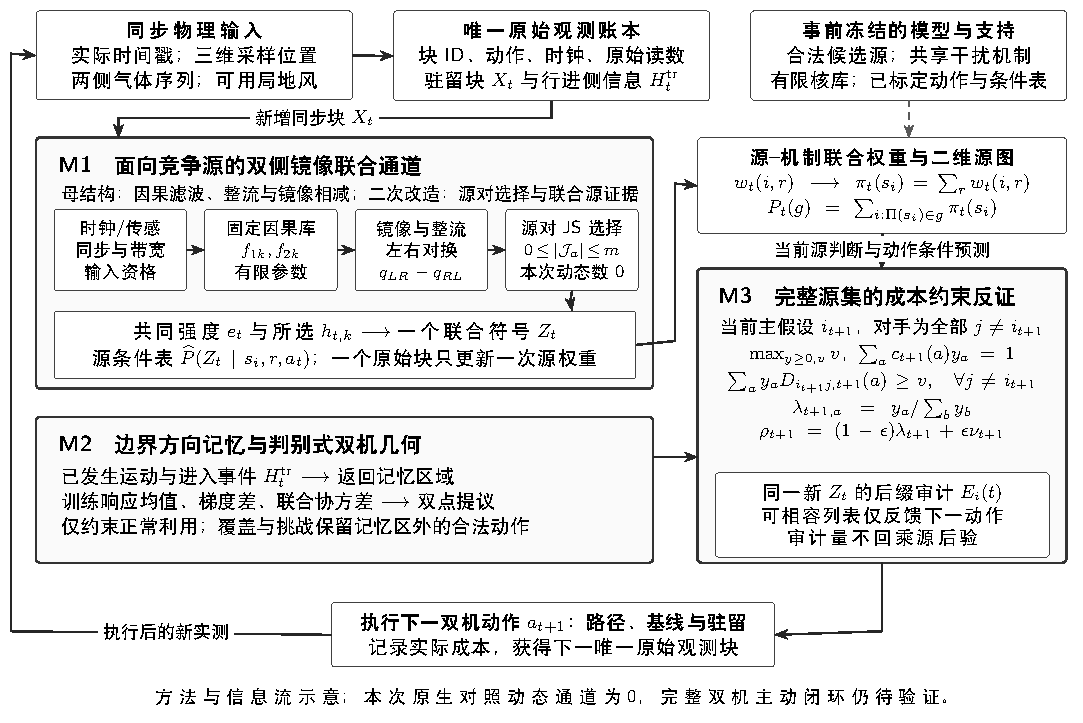
\includegraphics[width=0.98\textwidth]{figures/fig3_v7_framework.pdf}
\caption{三个模块的统一信息关系。完成第$t$块观测后规划第$t+1$步动作。依据V7可编辑方法图第2页重绘并修订，统一共享干扰机制$r$及主假设对完整竞争源的成本分配。M1产生联合观测符号，M2提出判别几何，M3选择有成本的反证动作；新观测后缀审计不回乘源后验。图示为方法设计，不表示完整原生闭环性能已验证。}
\label{fig:framework}
\end{figure*}

图\ref{fig:framework}中，M1将同步块转换为共模与镜像响应的联合符号$Z_t$，更新源--机制联合权重并边缘化输出$P_t(g)$；M2利用已发生的边界事件、运动方向及训练源响应形成合法双机动作；M3比较完整源集上的动作条件差异，计入实际成本，并以新后缀检查当前源解释。原始观测、几何记忆、源后验和审计量各有不同含义，不能互作独立气体证据重复计数。

设$Z_t=\phi(X_t)$为固定后或以过去信息选定的确定性编码，由数据处理不等式\ccite{Cover2006}
\begin{equation}
 I(S;Z_t\mid a_t,\mathcal F_{t-1})
 \le I(S;X_t\mid a_t,\mathcal F_{t-1}).
 \label{eq:dpi}
\end{equation}
因此M1不会创造原始观测中不存在的源信息。其待检验价值是在有限样本与有限模型容量下保留可泛化的判别结构，或者降低同等判别质量所需的标定与计算成本。M2通过实际改变测量位置和双机基线，才可能改变可获得的原始信息；M3控制这些动作的分配及已有判断的复核。三模块的设计完整性、条件性数学成立和实际性能验证分别报告，不以其中一项替代另外两项。

% V8 research manuscript method draft. Audited against V7 frozen commit
% 061ecf5ddea0a59dcf932b5038ad646b7af454a4. No new performance experiment.
% Citation keys are coordinated with the parent and may be remapped.

\section{面向竞争源判别的双侧镜像嗅觉计算}
\label{sec:m1}

本节研究如何在相同原始观测和有限标定样本下构造源判别表示。Brudner等的双侧嗅觉研究以羽流中心线侧别判断为任务，通过可学习因果时间滤波器、非线性整流和左右镜像相减提取互补线索，并经sigmoid形成侧别预测\ccite{Brudner2026Opponent}。本文保留其前端算子结构，将侧别输出改为竞争源条件下的联合观测分布，并用源对分离目标选择有限通道。镜像滤波、JS散度及贝叶斯归一化均有既有来源；本文拟验证的改造在于三者面向候选源判别的具体组合与选择机制。当前实现采用固定有限核库，尚未实现原母文的自由滤波器学习，也尚未获得优于完整联合观测的原生定位证据。

\subsection{双侧读出、真实时钟与因果镜像算子}

第$t$次同步测量的完整原始块为式\eqref{eq:block}的$X_t$。M1取其浓度与时钟投影$W_t=\{(\tau_{t,n},y_{t,n}^{L},y_{t,n}^{R})\}_{n=1}^{N_t}$，其中$\tau_{t,n}$为严格递增的物理秒值，记$+\equiv L$、$-\equiv R$，分别对应实际配对位置$\mathbf x_{t,n}^{L}$和$\mathbf x_{t,n}^{R}$。通道顺序在训练和测试中固定。原始浓度首先变换为
\begin{equation}
\xi_{t,n}^{\pm}=\log\!\left(1+\frac{[y_{t,n}^{\pm}-b_0]_+}{c_0}\right),\qquad c_0>0,
\label{eq:m1_preprocess}
\end{equation}
其中$[x]_+=\max(x,0)$，背景$b_0$和尺度$c_0$仅由事前配置或训练资料确定。该变换限制大幅值对有限样本估计的影响，但可能丢失低于背景的变化，不能视为无损预处理。

对$N_t>1$，记$\Delta\tau_t=\tau_{t,N_t}-\tau_{t,1}$，采用梯形求积权重
\begin{equation}
\omega_{t,n}=\begin{cases}
(\tau_{t,2}-\tau_{t,1})/(2\Delta\tau_t),&n=1,\\
(\tau_{t,n+1}-\tau_{t,n-1})/(2\Delta\tau_t),&1<n<N_t,\\
(\tau_{t,N_t}-\tau_{t,N_t-1})/(2\Delta\tau_t),&n=N_t.
\end{cases}
\label{eq:m1_time_weights}
\end{equation}
单快照的权重取1。共同强度与静态左右差异分别为
\begin{equation}
e_t=\sum_n\omega_{t,n}\frac{\xi_{t,n}^{+}+\xi_{t,n}^{-}}2,
\qquad
g_t=\sum_n\omega_{t,n}\frac{\xi_{t,n}^{+}-\xi_{t,n}^{-}}2.
\label{eq:m1_even_gradient}
\end{equation}
梯形加权仅实现真实时钟下的时间平均，不能恢复归档中缺失的高频变化。

以$\Xi_t^\pm=(\xi_{t,1}^\pm,\ldots,\xi_{t,N_t}^\pm)^{\mathsf T}$表示变换后序列。母算子的抽象形式是对左右序列施加两个共享时间滤波器，再以相同偏置整流和镜像相减：
\begin{equation}
\begin{aligned}
q_k(\Xi^+,\Xi^-)&=[\langle f_{1k},\Xi^+\rangle+
\langle f_{2k},\Xi^-\rangle+b_k]_+,\\
h_{t,k}&=q_k(\Xi_t^+,\Xi_t^-)-q_k(\Xi_t^-,\Xi_t^+).
\end{aligned}
\label{eq:m1_mirror}
\end{equation}
\begin{figure*}[t]
\centering
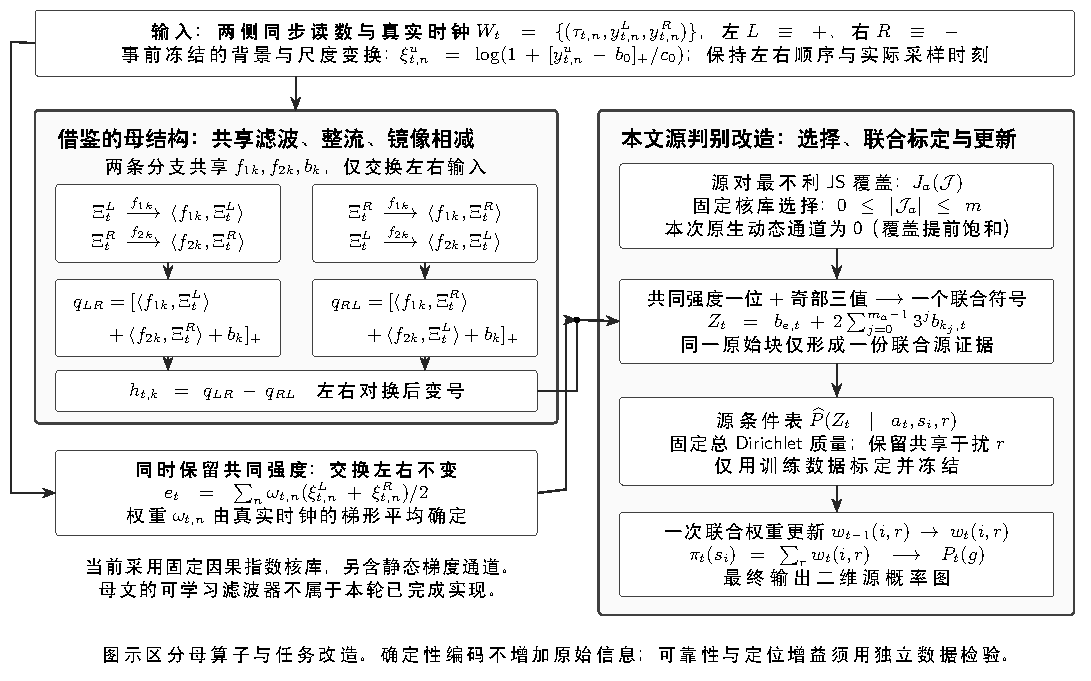
\includegraphics[width=0.98\textwidth]{figures/fig4_mirror.pdf}
\caption{M1的镜像内部运算与源条件证据。两路共享滤波器和偏置，交换左右输入后分别整流，再相减形成反对称响应；共模强度与选中响应只编码为一个联合符号。母算子结构与本文的竞争源选择、联合标定和概率输出分开标识；当前原生选择没有动态镜像通道。}
\label{fig:mirror}
\end{figure*}
式\eqref{eq:m1_mirror}中的滤波、整流和镜像差分属于母方法结构。其反对称性由交换两输入立即得到：$h_k(\Xi^-,\Xi^+)=-h_k(\Xi^+,\Xi^-)$；共同强度$e_t$在交换后不变。这一结构性质不意味着有限训练数据拟合的源条件概率也自动满足空间镜像对称。

当前V7将滤波器限制为因果指数核族\ccite{V7Archive}。设末端时刻$T=\tau_{t,N_t}$，延迟为$\ell_k\ge0$，衰减尺度为$\gamma_k>0$，则
\begin{equation}
\begin{aligned}
w_n^{(\ell_k)}&=
\frac{\mathbf1\{\tau_{t,n}\le T-\ell_k\}
e^{(\tau_{t,n}-T+\ell_k)/\gamma_k}\delta_n}
{\sum_m\mathbf1\{\tau_{t,m}\le T-\ell_k\}
e^{(\tau_{t,m}-T+\ell_k)/\gamma_k}\delta_m},\\
f_{1k}&=w^{(0)}-\eta_k w^{(\ell_k)},\qquad f_{2k}=-w^{(0)},
\end{aligned}
\label{eq:m1_restricted_bank}
\end{equation}
其中$\delta_1=\tau_{t,2}-\tau_{t,1}$，$\delta_n=\tau_{t,n}-\tau_{t,n-1}$（$n\ge2$），$\eta_k$为抑制系数。该离散核与式\eqref{eq:m1_time_weights}采用不同的明示求积规则；历史不支持所需延迟时拒绝计算。核库$\mathcal C$还包含式\eqref{eq:m1_even_gradient}的静态梯度通道。其有限参数、核数和选择规则属于当前实现，不应写成已经学习得到的动物最优滤波器。

传感器响应是输入资格的一部分。式\eqref{eq:sensor}的一阶、无噪声特例可写为$\widetilde y_n^{\pm}=a_n^{\pm}\widetilde y_{n-1}^{\pm}+(1-a_n^{\pm})C_n^{\pm}$，其中$a_n^{\pm}=\exp[-(\tau_n-\tau_{n-1})/\tau_s^{\pm}]$，$C_n^{\pm}$为受体处物理浓度。该关系说明需要标定的响应因素，并非本轮已经执行的真实传感器拟合。两侧响应时间、管路延迟和时钟偏差不相同，可能产生没有空间运动对应的镜像响应。因此，动态分支要求响应标定、同步位置和足够采样带宽；V7另外检查时钟误差与差分传感器延迟之和小于正滞后$\ell_k/3$。该比例是实现门限，不能替代物理带宽校准。

\subsection{源条件联合编码与通道选择}

每个动作$a$在训练数据上冻结共同强度中位数阈值$\theta_{e,a}$和各奇部绝对响应的0.4分位数阈值$\theta_{k,a}$，后者设置数值下限。若选中集合$\mathcal J_a=(k_0,\ldots,k_{m_a-1})$，则一个原始块仅编码为一个联合符号：
\begin{equation}
\begin{aligned}
b_{e,t}&=\mathbf1\{e_t>\theta_{e,a}\},\\
b_{k,t}&=1+\mathbf1\{h_{t,k}>\theta_{k,a}\}
-\mathbf1\{h_{t,k}<-\theta_{k,a}\},\\
Z_t&=b_{e,t}+2\sum_{j=0}^{m_a-1}3^j b_{k_j,t},\qquad O_a=2\cdot3^{m_a}.
\end{aligned}
\label{eq:m1_joint_symbol}
\end{equation}
这里$b_{e,t}$仅保留一位共同强度，不能表述为完整浓度信息得到无损保留。奇部采用关于零对称的三值量化；所有派生量共同进入一个符号，避免把同一块的强度、梯度和镜像响应当成相互独立的多次气体证据。

令$r\in\mathcal R$表示整段共享的有限干扰状态，包括事前声明的释放、传播或响应参数。每个动作、源$s_i$和状态$r$具有$K$个训练块，联合符号计数为$N_{a,i,r}(z)$。采用总质量固定为$\alpha_D>0$的Dirichlet平滑：
\begin{equation}
\widehat P_{\mathcal J}(z\mid a,s_i,r)=
\frac{N_{a,i,r}(z)+\alpha_D/O_a}{K+\alpha_D}.
\label{eq:m1_joint_law}
\end{equation}
不同动作的字母表可补齐到统一张量，但不可到达的补齐符号保持零概率。若保持已有分区不变并新增一个三值通道，则对新增坐标求和恰好返回原估计表，因为$\sum_{b=0}^2\alpha_D/(3O_a)=\alpha_D/O_a$。这排除了通道数增加同时隐式增加平滑总质量的混淆；平滑质量也并不因此获得真实误差概率解释。

通道选择以竞争源对为单位，采用不同干扰状态下的最不利JS距离：
\begin{equation}
\begin{aligned}
d_{ij}(\mathcal J,a)&=\min_{r,r'\in\mathcal R}
\operatorname{JS}\!\big(\widehat P_{\mathcal J}(\cdot\mid a,s_i,r),\\
&\hspace{4.3em}\widehat P_{\mathcal J}(\cdot\mid a,s_j,r')\big),\\
J_a(\mathcal J)&=\sum_{i<j}\min\{d_{ij}(\mathcal J,a),\kappa\}.
\end{aligned}
\label{eq:m1_cover}
\end{equation}
JS散度使用自然对数。以共同强度编码为起点，每轮选择使$J_a$增量最大的未选通道，并在增量不超过$\varepsilon_J$、达到通道上限或全部源对达到阈值$\kappa$时停止。最不利状态比较用于训练目标，不表示在线推断可在每个窗口任意更换固定干扰参数。

\paragraph{算法1（V7源对覆盖标定与在线编码）}
\begin{enumerate}
\item 仅访问训练实现，核验时钟、观测单位、传感器顺序和位置；计算共同强度及核库响应，冻结量化阈值。
\item 对每个动作令$\mathcal J_a=\varnothing$；计算式\eqref{eq:m1_joint_law}--\eqref{eq:m1_cover}。按最大正增量逐项加入通道，并保存每轮增益与停止原因。
\item 冻结动作映射、核库、阈值、联合条件表和训练文件标识。开发数据不参与上述任一步骤。
\item 在线接收新原始块，使用其实际时钟编码式\eqref{eq:m1_joint_symbol}；输出动作编号、唯一块编号及一个$Z_t$，交由共享后验更新一次。
\end{enumerate}

\subsection{联合源推断、信息边界与已发现的退化}

记$w_t(i,r)$为源和共享干扰状态的联合权重。在对应条件观测模型成立时，更新式为
\begin{equation}
\begin{aligned}
w_t(i,r)&=\frac{w_{t-1}(i,r)
\widehat P_t(Z_t\mid a_t,s_i,r,\mathcal F_{t-1})}
{\sum_{j,r'}w_{t-1}(j,r')
\widehat P_t(Z_t\mid a_t,s_j,r',\mathcal F_{t-1})},\\
\pi_t(s_i)&=\sum_r w_t(i,r).
\end{aligned}
\label{eq:m1_posterior}
\end{equation}
二维源图由式\eqref{eq:projection}得到。对共享$r$维持联合权重，避免每次以相同初始先验重新积分干扰状态。当前代码使用固定有限条件表，并主要以驻留块更新工作后验；行进期气体事件另用于M2动作提议。因此，除非进一步建立包含所有已见侧信息的正确条件模型，不能将其称为对完整行进与驻留数据的精确后验。时间窗口不重叠只解决重复使用原始样本的问题，并不自行证明窗口条件独立；重叠窗口必须采用与依赖关系相符的条件增量。

M1遵守式\eqref{eq:dpi}的数据处理边界；从$X_t$提取$W_t$再确定性编码也不会增加信息。可能的改进在于有限样本、模型容量或通信预算下更可靠地估计源判别表示；真正改变可获取观测信息的是下一节的动作选择。固定总平滑且编码分区嵌套时，经验联合JS不小于其边缘JS，因而式\eqref{eq:m1_cover}单调；但特征协同信息可使单个新增通道的增益为零，故不存在一般的次模、贪心全局最优或最小通道数保证。

原生开发实验已经暴露另一种明确退化\ccite{V7Native}：该实验只有两个已标定源，即一个源对；共同强度初始训练JS约为0.242586，已超过$\kappa=0.04$，截断目标随即达到0.04。任何新增通道的目标增量均为零，实际选择集合为空。由此评估的M1只剩共同强度编码，未使用动态镜像通道。此事实说明训练覆盖目标与留出判别目标之间存在落差；不能把相应负结果归因于双机几何已经被独立证伪，也不能通过改写论文将其当作已修复。

对于下一版本，可以研究以源条件预测损失替代硬截断覆盖或学习受因果及镜像约束的核，但这些均属待实现、待前瞻验证的设计。本文不改变已冻结阈值，不追改首轮成绩，也不以“强制加入一个动态通道”作为获得定位收益的证明。未见源的条件预测能力同样尚未由当前有限表建立。

\subsection{计算复杂度与适用条件}

设动作数$N_a$、源数$N_s=|\mathcal S|=J$、干扰状态数$N_r$、核库大小$|\mathcal C|$、代表性块长$N$、最大选中通道数$m$。全部训练特征提取约为$O(N_aN_sN_rK|\mathcal C|N)$；贪心至多评估$N_am|\mathcal C|$个候选集合，每次需要计数并计算$O(N_s^2N_r^2\,2\cdot3^m)$的源对距离。当前限制$m\le3$，仍须面对字母表随通道数指数增长的样本需求。在线实现计算整个核库，复杂度为$O(|\mathcal C|N)$，随后后验更新为$O(N_sN_r)$。上述复杂度不包含原生传播模拟、传感器响应标定和飞行成本。

\section{判别式双机测量与持续反证定位}
\label{sec:m2m3}

M1处理给定窗口中的信息表达，M2与M3共同决定下一窗口的获取方式。M2以气味边界的返回方向生成可执行测量提议，再用竞争源响应差设计双点几何；M3在完整合法源集上分配测量成本，并用独立于旧源赔率的新观测后缀审查当前假设。两模块均已有研究原型\ccite{V7Archive}，但正式原生双无人机主动实验尚未执行\ccite{V7Native}；本节的模型与条件性质不能替代该性能证据。

\subsection{M2：动态边界方向记忆与返回区域}

Siliciano等研究了由气味边界进入、退出事件与运动方向构成的嗅觉导航策略\ccite{Siliciano2026Vector}。本文将方向记忆用于动作候选生成，而不把记忆向量作为第二份源似然。对经过时钟与响应延迟校正的进入事件$k$，令$\widehat{\mathbf d}_k$为真实已观察运动窗口内速度积分后归一化的方向，更新
\begin{equation}
\begin{aligned}
\mathbf m_{k+1}&=a_m\mathbf m_k+b_m\widehat{\mathbf d}_k,\\
\Sigma_{m,k+1}&=a_m^2\Sigma_{m,k}+b_m^2V_k,\qquad
\mathbf u_t=\frac{\mathbf m_t}{\|\mathbf m_t\|}.
\end{aligned}
\label{eq:m2_memory}
\end{equation}
$V_k$包含窗口内方向散布、声明的方向噪声，以及已有有效记忆时新方向与旧记忆单位方向之差的外积项；该递推是忽略跨事件相关项的工程不确定性近似，未被校准为真实协方差。$b_m$不要求等于$1-a_m$。记$k(t)$为截至决策$t$已经完成的合格进入更新次数，后文$\mathbf m_t=\mathbf m_{k(t)}$及$\Sigma_{m,t}=\Sigma_{m,k(t)}$。运动方向来自位置变化及对应段的实际行进方向，不能用机头朝向代替。静止时羽流扫过传感器不建立该运动记忆；方向相消或历史过期时不输出有效返回方向。当前无风版本只更新进入记忆，有风版本增加退出方向和上风门控，仍不等同于母文完整随机运动模型的复现。

现有解析控制演示以两机浓度算术均值大于0.3作为组级气味事件，阈值单位属于该解析后端，并把事件配对到两机位置均值的平面运动。它不等于两机中心处的实测气体，也不证明两机在同一时刻穿越同一物理边界。原生任务中，两侧异步进入、组级事件合成、阈值与响应延迟仍须独立标定；本稿不把这一演示规则写成已经验证的原生边界探测器。

对$\|\mathbf m_t\|>0$，归一化的Jacobian为$J_m=(I-\mathbf u_t\mathbf u_t^\top)/\|\mathbf m_t\|$，方向不确定性矩阵近似为$\Sigma_u=J_m\Sigma_{m,t}J_m^\top$。以当前两机位置均值的平面投影$\bar{\mathbf x}_t\in\mathbb R^2$为原点，取单位法向$\mathbf n_t\perp\mathbf u_t$，定义有限返回区域
\begin{equation}
\begin{aligned}
\mathcal T_t&=\{\bar{\mathbf x}_t+s\mathbf u_t+\zeta\mathbf n_t:\\
&\hspace{2em}0\le s\le L_T,\ |\zeta|\le R_t(s)\},\\
\Sigma_T(s)&=\Sigma_x+q_m\Delta t_m I+(v_{\max}\sigma_\tau)^2I+s^2\Sigma_u,\\
R_t(s)&=r_0+k_T\sqrt{\mathbf n_t^\top\Sigma_T(s)\mathbf n_t}.
\end{aligned}
\label{eq:m2_tube}
\end{equation}
其中$\Delta t_m$是记忆物理年龄，$q_m$为位置漂移方差率，$\sigma_\tau$为延迟不确定度。该区域是工程不确定性传播结果，尚未校准为某个概率覆盖水平。它随当前位置平移，保留相对返回方向，不把上次边界坐标当成静止目标；也不承担源概率更新或安全航路认证。

\subsection{M2：面向竞争源响应差的双点几何}

当前几何接口在共同测量高度上设计平面中心$\mathbf q$、间距$d$和单位基线方向$\mathbf u$，两测点为$\mathbf q\pm d\mathbf u/2$。三维位置仍由任务数据合同记录，但本文不将该平面接口扩写成已实现的一般三维编队控制。由训练实现或在线因果可得模型提供源$s_i$的原始有限窗均值$\mu_i(\mathbf q)$、空间梯度$\nabla\mu_i(\mathbf q)$和偶奇联合协方差$\Sigma_i(a)$。这些量不读取未观测测试全场；其原始浓度尺度与M1的对数编码分开。

在合法局部半径内，一阶双点响应预测为
\begin{equation}
\bar{\mathbf z}_i(a)=
\begin{bmatrix}\mu_i(\mathbf q)\\
\frac d2\mathbf u^\top\nabla\mu_i(\mathbf q)\end{bmatrix},
\quad
\Delta\mathbf z_{ij}(a)=\bar{\mathbf z}_i(a)-\bar{\mathbf z}_j(a),
\label{eq:m2_response}
\end{equation}
并以完整联合协方差形成设计距离
\begin{equation}
D_{ij}^{\mathrm{geom}}(a)=
\Delta\mathbf z_{ij}^{\top}
[\Sigma_i(a)+\Sigma_j(a)+\lambda_gI]^{-1}
\Delta\mathbf z_{ij}.
\label{eq:m2_geometry_score}
\end{equation}
$\lambda_g\ge0$为事前声明的正则量，不能利用开发结果反复调节。池化矩阵必须正定；当前代码在不满足时拒绝输入，要求提供合格方差或明确正则量，不静默使用伪逆。式\eqref{eq:m2_geometry_score}不是气体似然、KL散度或审计统计量；协方差的交叉项只使用一次。当前训练接口采用普通RBF拟合均值及解析梯度，该适配本身不作为新算法贡献，且外推与协方差池化仍需独立校准。

上述几何有明确适用边界。若局部Hessian范数有界$\|\nabla^2\mu_i\|\le M_i$，双点精确偶部与$\mu_i(\mathbf q)$、精确奇部与一阶梯度项的误差均不超过$M_id^2/8$。这由两端Taylor余项相加、相减得到；当前接口检查局部半径，却没有实测证明$M_i$界。长基线应采用精确端点预测，不能借短基线展开赋予其资格。当两源均值相等、联合协方差不随方向变化且梯度差$\Delta\mathbf g\ne0$时，式\eqref{eq:m2_geometry_score}由$\mathbf u=\pm\Delta\mathbf g/\|\Delta\mathbf g\|$最大化；梯度差为零时各方向并列。方向相关噪声、成本及可达性存在时须共同比较。

当前M1的阈值与联合条件表按有限动作编号标定，因此M2实际执行的动作须落在事前安装集合$\mathcal A^{\rm inst}$内，并与其位置、传感器、时钟及读出定义一致。RBF可计算新几何的均值和梯度提议，但不会自动为新动作生成合格的M1联合似然。未安装的中心、基线或方向仍需独立动作标定及冻结，或经验证的参数化条件预测接口；当前原型没有自动完成这一步。

M2枚举已安装且通过端点合法性、间距和线性化半径检查的动作，输出全部动作与源对的设计距离矩阵。记当时合法且剩余预算可负担的集合为$\mathcal A_t^{\rm legal,aff}\subseteq\mathcal A^{\rm inst}$，M2利用掩码形成$\mathcal A_t^{\rm use}\subseteq\mathcal A_t^{\rm legal,aff}$。返回区域内存在超过判别阈值的动作时，优先提出这些动作；否则开放区域外的合法复测。某个均值型距离为零不代表完整观测分布不可区分，高阶结构和协方差差异仍可能有用。返回区域及利用掩码不能禁止M3在$\mathcal A_t^{\rm legal,aff}$内的覆盖和显式挑战。现有代码的端点检查也不自动证明整段航路无碰撞或两机同步到达。

\subsection{M3：完整源集上的成本分配与持续覆盖}

\begin{figure*}[t]
\centering
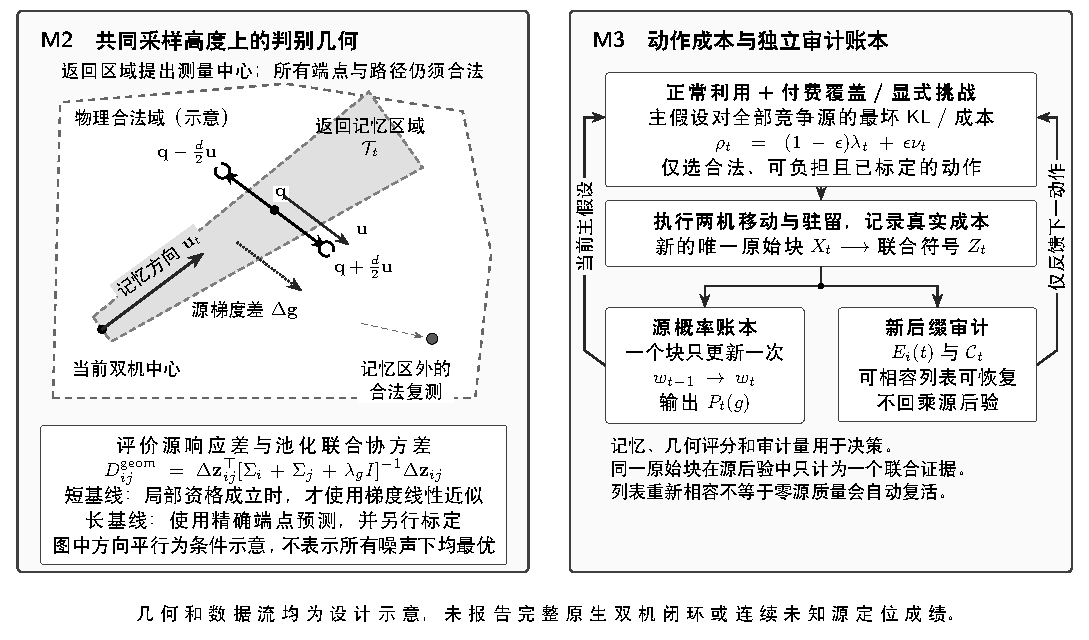
\includegraphics[width=0.98\textwidth]{figures/fig5_geometry_audit.pdf}
\caption{双机判别几何与持续反证决策示意。左侧为共同高度下的返回区域、中心与双点基线，响应差分数仅用于动作设计；返回区域外的合法测量仍可被覆盖或挑战。右侧为新观测进入一次后验更新与独立后缀审计，审计只反馈下一动作。全部动作须具备相同编号下已标定的条件预测，几何示意不是原生飞行验证。}
\label{fig:geometry}
\end{figure*}

主动序贯假设检验提供了按竞争假设差异分配测量的理论基础\ccite{Hsu2025Tradeoffs}，非同质成本研究进一步区分测量次数与资源消耗\ccite{Vershinin2026Costs}。本文沿用这些目标结构，研究其与低后验候选持续复核、M2区域外挑战和新后缀审计的结合，不将KL、线性规划或Chernoff原则本身列为原创。

给定当前最大工作后验源$i_t=\arg\max_i\pi_{t-1}(s_i)$，先从联合权重得到用于规划的干扰条件权重
\begin{equation}
\begin{aligned}
\beta_{ir,t}&=\begin{cases}
w_{t-1}(i,r)/\pi_{t-1}(s_i),&\pi_{t-1}(s_i)>0,\\
\beta_{ir,0},&\pi_{t-1}(s_i)=0,
\end{cases}\\
p_{i,t}^{a}(z)&=\sum_r\beta_{ir,t}\widehat P(z\mid a,s_i,r).
\end{aligned}
\label{eq:m3_predictive}
\end{equation}
其中$\beta_{ir,0}$为安装模型对源$s_i$的归一干扰先验。零源质量时退回该先验，只用于提出反事实测量，不给工作后验补回源质量。当前程序中的$\widehat P$是冻结有限表；此处预测不因此成为对全部行进历史的真实条件律。源对分离及动作成本定义为
\begin{equation}
D_{ij,t}(a)=\sum_zp_{i,t}^a(z)\log\frac{p_{i,t}^a(z)}{p_{j,t}^a(z)},\qquad c_t(a)>0.
\label{eq:m3_kl}
\end{equation}
$c_t(a)$应包括到位、恢复、稳定和同步采样的完整成本。由安装表计算的KL属于模型内设计量，不能当作真实未知羽流信息率的校准下界。以所有$j\ne i_t$为对手，在非空利用域$\mathcal A_t^{\rm use}$上求
\begin{equation}
\max_{\lambda\in\Delta(\mathcal A_t^{\rm use})}
\frac{\min_{j\ne i_t}\sum_a\lambda_aD_{i_tj,t}(a)}
{\sum_a\lambda_ac_t(a)}.
\label{eq:m3_cost_ratio}
\end{equation}
本式及下式的动作求和均在$\mathcal A_t^{\rm use}$内。令$y_a=\lambda_a/(\sum_b\lambda_bc_t(b))$，可等价转为
\begin{equation}
\begin{aligned}
\max_{y\ge0,v}\quad&v,\\
\mathrm{s.t.}\quad&\sum_ac_t(a)y_a=1,\\
&\sum_ay_aD_{i_tj,t}(a)\ge v,\quad j\ne i_t;\\
&\lambda_a=\frac{y_a}{\sum_by_b}.
\end{aligned}
\label{eq:m3_lp}
\end{equation}
由$\lambda$到$y$及反向归一化均保持式\eqref{eq:m3_cost_ratio}的值，给出等价性。求解后以零概率延拓到$\mathcal A_t^{\rm legal,aff}$。实现内部可用资源份额$c_t(a)y_a$求解，但抽样频率必须按$y$归一化，不能直接使用资源份额。两源情形只有一个对手约束，退化为选择最大$D/c$的动作，因此两源固定探针实验不能验证多候选分配机制。

为使低后验源仍有机会得到反证性测量，执行分布定义为
\begin{equation}
\rho_t(a)=(1-\epsilon)\lambda_t(a)+\epsilon\nu_t(a),
\qquad 0<\epsilon\le1,
\label{eq:m3_coverage}
\end{equation}
其中$\nu_t$在$\mathcal A_t^{\rm legal,aff}$上预先定义，并与源后验无关；完整版默认取均匀正覆盖。若该集合为空，则结束当前预算内采样，不再求分配或生成观测。M2仅限制正常利用分配，覆盖及显式挑战可访问利用域外的合法可负担动作。当最坏信息率未超过事前数值容差、利用域为空、支持不匹配造成无限KL或审计指定挑战源$j$时，当前原型转用$\min\{D_{i_tj,t}(a),D_{ji_t,t}(a)\}/c_t(a)$在$\mathcal A_t^{\rm legal,aff}$上选择源对挑战，仍保留覆盖分量。无显式挑战时，程序在具有正双向分离的对手间轮转；若不存在，则在全部对手间轮转。若所选源对的最佳分数仍未超过容差，利用分布也设为$\nu_t$，最终$\rho_t=\nu_t$。这些回退是明示工程规则，不继承完整线性规划最优性。

在固定合法动作域上，若$\nu(a)>0$且连续执行$T$步，则由每步条件概率下界可得
\begin{equation}
\Pr\{N_a(T)=0\}\le[1-\epsilon\nu(a)]^T.
\label{eq:m3_coverage_bound}
\end{equation}
该界说明错误后验不会关闭动作$a$的访问概率；它不证明动作可辨、有限预算必然恢复或估计KL准确。预算尾段动作被移除时，应报告实际可负担集合，不能延用固定全域的无限期保证。覆盖每步的期望成本为$\epsilon\sum_a\nu_t(a)c_t(a)$，并非免费探索。

\subsection{M3：新后缀审计与可恢复候选列表}

旧观测可能形成错误高置信，因而审计从只依赖已见信息的时刻$t_0$开始，所有源--干扰状态的后缀似然初始化为1，不继承旧源赔率。可预测替代分布与复合零假设最大似然的结构已有统计学基础\ccite{Wasserman2020Universal}，近期量子序贯检验给出其另一领域应用\ccite{Zecchin2025QSUT}。这里仅借鉴已读取作者稿中的统计结构，不涉及量子硬件，也不将其量子任务实验当作气源定位验证。

对固定共享状态$r$定义
\begin{equation}
\begin{aligned}
L_{ir}(t)&=\prod_{k=t_0+1}^{t}
P_k(Z_k\mid s_i,r,a_k,\mathcal F_{k-1}),\\
Q_{-i}(t)&=\sum_{j\ne i,r}w_{jr}^{(-i)}L_{jr}(t),
\end{aligned}
\label{eq:m3_suffix}
\end{equation}
其中$w_{jr}^{(-i)}>0$在审计前固定、对$j\ne i,r$归一化。当$Q_{-i}(t-1)>0$时，由后缀混合得到下一结果出现前冻结的替代预测
\begin{equation}
\begin{aligned}
q_{-i,t}(z)&=\sum_{j\ne i,r}
\frac{w_{jr}^{(-i)}L_{jr}(t-1)}{Q_{-i}(t-1)}\\
&\hspace{3em}\cdot P_t(z\mid s_j,r,a_t,\mathcal F_{t-1}),\\
E_i(t)&=\frac{Q_{-i}(t)}{\max_rL_{ir}(t)}.
\end{aligned}
\label{eq:m3_evalue}
\end{equation}
分母对整段相同$r$的似然取最大值，不能改为逐时刻分别取最大后相乘。若$Q_{-i}(t-1)=0$，下一步可选择任意非负且和为1的替代预测，当前程序取字母表上的均匀分布；但累计替代路径质量继续保持零，不因重新归一化而复活。所有安装状态均不能解释整个后缀时，报告模型支持失败，不以人为概率下限产生一个认证赢家。对模型概率统一添加下限会改变零假设族和检验律，必须重新校准，不能声称原风险结论无条件保留。

\paragraph{条件性质（模型内真源覆盖）}
若真源$s_i$和一个固定真干扰状态$r_*$均在安装族中；$P_k$是给定同一实际过去及动作的真实正规条件律；动作、审计起点和替代预测仅使用过去；且原始观测不被重复当作新条件增量，则
\begin{equation}
\Pr_{s_i,r_*}\{\exists t\ge t_0:E_i(t)\ge1/\alpha_A\}\le\alpha_A.
\label{eq:m3_risk}
\end{equation}
证明如下：$\max_rL_{ir}\ge L_{ir_*}$，故$E_i\le M_t=Q_{-i}/L_{ir_*}$。正规可预测的替代分布使$M_t$为非负检验超鞅；在共同支持上，每步似然比的条件期望不超过1。由Ville不等式得到$M_t$的越界概率界，点态支配再得到式\eqref{eq:m3_risk}。$E_i$自身不必为超鞅。该性质是对标准似然比工具在当前有限族中的适配证明，不是新发明的概率不等式。

训练拟合的直方图或Gaussian并不自动满足真实条件族包含性；当前审计只有模型内解释。即使拟合算法在每次观测前冻结，也仍需独立证明校准和时间依赖处理；仅有可预测性并不足以获得物理风险保证。多个审计重复启动还须分配累计错误预算。原生环境中的传感器失配、未见风场与连续干扰状态覆盖均待验证。

当前可相容集与从未越界集分别为
\begin{equation}
\begin{aligned}
\mathcal C_t&=\{s_i:E_i(t)<1/\alpha_A\},\\
\mathcal C_t^{\mathrm{ever}}&=
\{s_i:\max_{t_0\le u\le t}E_i(u)<1/\alpha_A\}.
\end{aligned}
\label{eq:m3_lists}
\end{equation}
前者允许重新进入，后者单调缩小；二者都不是源概率分布。若当前最大后验源不在$\mathcal C_t$，原型从仍相容的替代源中选择审计量最小者作为下一次显式挑战。此反馈只改变动作提议，不修改旧源概率，不将$E_i$或其倒数重新乘入式\eqref{eq:m1_posterior}。因此，同一原始块可以分别用于后验计算和决策审查，但在源后验中只计入一次。所有源仍须保留于合法候选支撑；初始质量为零或已由结构零永久消去的源不能靠乘法更新恢复。

\subsection{模块接口、伪代码与区别于普通信息增益的作用}

普通期望信息增益根据后验加权的平均熵下降选择动作；M2提供由方向记忆和响应差生成的几何提议，M3正常分配关注当前主假设对全部竞争源的最坏单位成本分离，并额外保留后验独立覆盖及审计触发的源对挑战。目标不同不意味着后者必然更优；必须在相同两机资源、相同原始信息权限和完整实际成本下与联合EIG比较。当前控制实现的行进信息仅进入M2，这一额外信息通道必须同时提供给强基线或单独消融。

\paragraph{算法2（统一测量与源概率更新）}
\begin{enumerate}
\item 初始化严格正的源先验$\pi_0$、归一干扰先验$\beta_{ir,0}$与联合权重$w_0(i,r)=\pi_0(s_i)\beta_{ir,0}$；冻结已安装动作、M1模型、传感器资格、资源预算及最大步数。初始化方向记忆与观测账本，指定单次审计错误预算$\alpha_A$，从$L_{ir}=Q_{-i}=1$启动审计。当前演示仅用一个账本；若另行设计重复启动，须事前分配累计错误预算。
\item 每轮根据已发生的运动与气味事件更新M2记忆，在已安装动作中构造利用域及合法可负担域。预算耗尽、达到预设步数或合法可负担域为空时结束循环。
\item 由当前联合权重计算源预测，针对全部合法源在利用域求成本分配，并在合法可负担域叠加付费覆盖；若旧主假设受到新后缀反证，则指定源对挑战。按明示回退规则处理空利用域及无正分离情形，并抽取下一动作。
\item 在新结果出现前冻结审计预测，执行移动、稳定与采样，记录两机位置、原始时钟、传感器标识、实际成本和唯一块编号。观测资格或时序核查失败时停止并报告原因，不插补新证据。
\item 调用M1产生一个联合符号，更新一次源--干扰权重并输出二维源图；在独立审计账本更新后缀似然和候选列表。若全部安装状态不支持观测或审计后缀，停止并报告模型支持失败，不据此认证某个源。
\item 核算实际资源消耗，将审计反馈用于下一动作后返回步骤2；派生记忆、规划分数和审计量不作为额外气体似然。结束时保存最后有效源图和诊断。审计列表只剩一个源不触发自动成功，也不等同于真实位置已经正确。
\end{enumerate}

若中心、间距、方向个数分别为$N_q,N_d,N_u$，M2几何评分约为$O(N_qN_dN_uN_s^2)$；当前方向历史采用列表保存和扫描，不能将整段实现宣称为常数时间。令$O=\max_a O_a$为统一补齐后的联合字母表大小，M3完整源对KL计算为$O(N_aN_s^2O)$，之后还需有限线性规划求解；审计预测混合约为$O(N_s^2N_rO)$，一次观测更新约为$O(N_sN_r)$。原型固定动作成本和返回共同起点的演示尚不覆盖一般时变航路成本；正式双机实验须统一规划成本、执行时间及审计记账，并独立验证路径和同步到达。

\section{预实验与后续验证方案}
\label{sec:experiments}
本节将已执行结果与待执行实验分开。已有结果来自冻结提交\texttt{061ecf5ddea0a59dcf932b5038ad646b7af454a4}及其原始收据\ccite{V7Native}；本轮仅核对、重排和复算已记录的统计量，没有生成新气体世界、训练新滤波器或启动机器人闭环。软件可运行、读出与旧实现一致以及定位性能改善分别评价。

\subsection{数据来源、划分和读出资格}
原生归档为House01中\texttt{1,3-2,4\_fast}设置的两个释放位置，每个位置4个独立实现，共8个世界。原始逐世界1803帧，总计14424帧，覆盖0--999.502991\,s，并逐帧核对SHA256。其环境属于VGR/GADEN研究数据背景\ccite{Ojeda2023VGR}，归档名称中的\texttt{s2x}表示移源世界，不是枫树岭S2湖岸数据。源A和源B的三维坐标分别为$(-0.60,1.95,0.40)$\,m与$(-0.40,-2.90,-0.30)$\,m，均经原三维地图核查处于自由体素。两源同时改变水平位置和高度，不能将响应差解释为纯水平位置干预。

各源的r01/r02用于TRAIN，r03/r04用于DEV，因此训练和开发均为4个世界。两侧探针沿用此前冻结的12/17号，每个探针实际为4个原生格中心浓度的均值；两个采样池中心间距约7.003\,m，不能称为理想无体积单点PID。窗口在读取浓度前固定为50--70\,s，实际含33帧，时间为50.2998047--69.4995117\,s，相邻帧约0.6\,s；没有插值补造高频运动。每个世界贡献一个窗口，33帧不是33个独立实验。

原V7核库要求最大间隔0.25\,s，不能直接用于上述归档。原执行记录在开发评分前另行冻结粗采样适配：最大间隔0.61\,s，延迟1.8/3/6\,s，衰减1.5\,s，保留镜像算子及选择规则。该适配只允许解释粗采样、理想零延迟浓度读出的结果，真实传感器响应标定标记仍为未通过。它不代表恢复了动物尺度的快速气味运动，也不代表双无人机动力学或旋翼干扰已经验证。

原执行回归包括30个探针、10个时刻和4个训练世界的1200项浓度查询，全部通过，其中485项非零，最大绝对差$3.5763\times10^{-7}$\,ppm。软件测试最终71/71通过；20项C++/Python模型推理对照的符号及候选后验一致，最大特征差$2.22\times10^{-16}$。这些结果支持归档读出与实现一致性，不证明真实物理分布准确、概率校准或气源定位有效。

\subsection{固定观测下的完整普通对照}
所有方法使用相同TRAIN/DEV世界、相同窗口和候选支持，模型及预处理在DEV评分前冻结。表\ref{tab:native}保留原始\texttt{R2\_RESULT.json}汇总中的全部11个比较项。Gaussian头按有限训练窗口拟合；完整raw-joint同时提供向量量化（VQ）和Gaussian对照，以避免只用弱离散基线衬托方法。这里的“完整”指该窗口中实际保存的两侧样本，不包含窗口外的气体全场。

\begin{table*}[t]
\centering\small
\caption{两已标定源、4个独立开发世界上的冻结原生浓度读出结果。全部为固定观测离线对照；没有原生PMFS或自主双机成绩。}
\label{tab:native}
\begin{tabularx}{\textwidth}{Y c c r p{4.3cm}}
\toprule
方法 & 严格正确/4 & 并列数 & 原记录MAP均误差/m & 结果解释\\
\midrule
普通单点时间均值 + Gaussian & 4 & 0 & 0 & 两候选的当前开发分类已饱和\\
普通单点完整时间窗 + Gaussian & 4 & 0 & 0 & 单侧时间序列的普通控制\\
普通双点时间均值 + Gaussian & 4 & 0 & 0 & 未比单点控制增加判对样本\\
完整双点窗口 raw-joint VQ & 4 & 0 & 0 & VQ码本因4个训练块缩减为4\\
完整双点窗口 + Gaussian & 4 & 0 & 0 & 强普通联合对照\\
母结构best-one + 原直方图 & 2 & 2 & $0^{\dagger}$ & 实际选中静态梯度，非母文完整学习模型\\
母结构所选特征 + Gaussian & 4 & 0 & 0 & 同一受限静态特征，更换统计头后全部判对\\
固定双通道 + 原直方图 & 2 & 2 & $0^{\dagger}$ & 两个样本依赖固定顺序破并列\\
共同强度even + 原直方图 & 2 & 0 & 2.427061 & 与空通道选择后的M1一致\\
M1源对覆盖 + 原直方图 & 2 & 0 & 2.427061 & 动态镜像通道选择数为0\\
M1所选特征 + Gaussian头 & 1 & 0 & 3.640591 & 更换头部未恢复普通对照表现\\
\bottomrule
\multicolumn{5}{p{\dimexpr\textwidth-2\tabcolsep\relax}}{\footnotesize $\dagger$ 原记录按固定候选顺序破并列，恰好得到0\,m；严格判对仍为2/4。该0不作为无歧义定位成功。其余0也只是当前两个已标定候选的离线分类零误差，不表示连续未知源达到零米精度。}\\
\end{tabularx}
\end{table*}

M1在两个源A开发世界中均选择源B，在两个源B世界中判对，平均平面误差为2.427061\,m。共同强度的训练JS约0.242586，超过覆盖阈值0.04；唯一源对已被截断目标判为覆盖，贪心第一轮增益为0，最终选择集合为空。该行为由训练收据和导出模型直接确认，M1成绩也与共同强度even对照一致。母结构受限特征在Gaussian头下为4/4，进一步表明表征与统计头的作用需要分别控制，但它仍不是原母文的可学习网络。由于动态镜像通道没有进入M1评分链，本结果检验的是当前选择与量化方案，不能解释为动态镜像核已被充分使用后仍无效。

普通单点时间均值已经全部判对，说明当前任务没有建立双点或动态关系的必要性；M1的失败也不能简单归结为双机几何不佳。相同测量中存在普通方法能够利用的源差，而当前压缩未稳定保留。该4世界小样本不支持稳定泛化、显著性或真实概率校准主张，更不能在基线误差为零的任务上计算相对误差改善10\%。当前有限条件表仅覆盖两个已标定位置，未验证未见源泛化。

此前静态pilot和解析控制后端仅提供不同层次的辅助记录。静态pilot的普通raw-joint为40/40、静态M1为31/40，但40张快照来自4个开发世界；解析控制矩阵包含156个episode，其普通强基线与完整方法最终端点均饱和\ccite{V7Archive}。它们不是本节原生动态对照的追加独立样本，也不作为原生双机闭环收益。当前M1未通过独立增益门，M2/M3正式原生主动实验按原合同未启动，保留原始首次结果。

\subsection{需要逐项回答的实验问题}
后续实验围绕三个独立命题设置，而不以整套方法胜过一个弱基线替代模块验证。命题H1为：在训练预算和模型容量相同的条件下，源判别镜像通道能否较普通完整联合观测及母结构适配获得稳定源排序、校准或样本效率收益。命题H2为：在两机资源相同的条件下，边界记忆结合响应差几何能否比普通重捕获与无记忆判别几何取得更有辨识力的测量。命题H3为：在相同原始流、运动约束和后验更新下，完整源覆盖与新后缀审计能否降低错误高置信持续时间、改善恢复，而不增加正常任务错误。

\begin{table*}[t]
\centering\small
\caption{正式实验矩阵与执行状态。待执行项使用明确占位，不预填优势曲线。}
\label{tab:plan}
\begin{tabularx}{\textwidth}{p{1.45cm}Y Y p{1.9cm}}
\toprule
实验层次 & 比较对象 & 主要控制与回答的问题 & 当前状态\\
\midrule
固定观测H1 & 普通均值、raw-joint、母核库best-one、固定等数量通道、M1、无共模/无镜像/无源对目标 & 相同同步窗口、同训练块数、相同头部与总平滑质量；时间打乱、左右交换、传感器延迟扰动分开 & 两源开发完成；跨源结果待补\\
母文迁移 & PNAS原可学习结构 + 源条件头、固定核库best-one & 区分原母网络学习能力、必要任务适配和本文源对选择；训练预算相同 & 精确迁移待实现/待验证\\
几何H2 & 普通边界返回、无记忆响应差、仅返回区域、完整M2 & 相同双机、候选动作及代价；分别检查间距、方向、返回记忆和区域外复测 & 原生结果待补\\
决策H3 & 联合EIG、直接成本Chernoff、无覆盖、无审计反馈、完整M3 & 相同M1/M2与全原始流；正常先验和预设错误先验分别测试 & 原生结果待补\\
完整定位 & 原生PMFS-1U、透明适配PMFS-2U、raw-joint+EIG、各模块消融、完整方法 & 固定轨迹与自主闭环分开；设备数、样本数、墙钟与两机总时间分别核算 & 全域原生成绩待补\\
迁移与实用性 & 未见源、风、独立传播实现、House01/02/03、合格S2 & 未见源需先具备参数化条件预测接口；真实可用局地风与全真风oracle分开 & 待执行；S2资格未完成\\
\bottomrule
\end{tabularx}
\end{table*}

PMFS-1U保留原生算法和固定设置，作为设备资源参照；PMFS-2U是需公开说明的双输入适配，不冒称已有官方双机实现。主算法比较应在相同两机输入上进行，另报单机资源消融。M1的母方法对照至少包含同核库best-one与原可学习结构的任务适配，两者不能混称精确母方法复现。普通完整联合模型可包含VQ、正则Gaussian及适当容量的时间模型；模型选择只使用独立训练/验证资料，不能反复查看最终测试后挑选有利基线。

H1首先使用同观测固定轨迹，比较表示对同一批证据的利用。H2/H3和完整方法随后在原生GADEN-RT、相同合法起点和预算下运行自主闭环，使策略真正改变后续位置。当前代码在行进期读取气体事件供M2使用、在驻留期更新源概率，因此公平对照必须给所有方法相同可用原始流，或对这一额外信息单独消融；仅把飞行时间相等不能消除信息权限差异。真实运动、稳定、恢复和采样均计入成本，不把两个同时工作的传感器计为一个。

\subsection{划分、指标与统计判据}
独立性以完整传播世界为基本单位。训练、调参验证和最终测试按源位置、风条件和实现标识预先分开，不能把同一世界的相邻窗口分到两侧充当独立样本。House01/02/03分别报告，不把源数、风数和实现数相乘成没有实际运行的全交叉样本量。未见源验证还要求源坐标到条件响应的参数化模型或经资格审查的在线前向接口；当前按源编号标定的有限表不具备该能力，补齐接口之前该项保持待执行。

源级结果至少包括严格Top-1、MAP距离、Top-5\%位置读出、真源平均秩及源对分离方向。定义$\mathcal M_t=\operatorname*{arg\,max}_{g}P_t(g)$；严格Top-1只有在真源单元为唯一最大项时记为正确，并列单独报告。Top-5\%沿用固定官方O24实现的空间读出与误差计算，正式测试前须一并冻结其代码版本、合法单元域、取整、权重及并列规则。本文保留B4原CSV值及已有独立复算值，不在尚未逐项核验该实现细节时自行添加同名公式。若另设概率加权位置指标，应另名、另报，不能替换或混称官方Top-5\%。

后验可靠性报告源级负对数评分、Brier评分和90\%最高后验密度区域覆盖，而非仅报告方差。对离散真源单元$g^*$，
\begin{equation}
 \begin{aligned}
  \mathrm{NLL}_t&=-\log P_t(g^*),\\
  \mathrm{BS}_t&=\sum_{g\in\mathcal G}
      \big[P_t(g)-\I\{g=g^*\}\big]^2.
 \end{aligned}
 \label{eq:evalscores}
\end{equation}
若$P_t(g^*)=0$，NLL应保留无限或明确报告预先登记的数值读出规则；不得靠事后平滑隐藏模型支持失败。错误高置信按预先固定的概率阈值与定位容差定义，报告发生率、持续时间、恢复代价及未恢复比例。官方\texttt{success}保留原定义单独记录，不作为真实位置成功的替代。

同一世界上的方法差采用配对统计，以独立世界而非窗口为重采样单位；跨源/风结论需按其分层报告并给出置信区间。试验规模由先验功效分析或预设置信区间宽度确定，不能依据开发集胜负追加种子。样本效率以相同测试集上的训练世界数量学习曲线评价；成本报告原始样本数、两机总飞行时间、墙钟时间、内存与前向计算次数，区分模拟器成本和算法成本。

研究目标为在非饱和、独立留出测试中，相对同权限强基线实现至少10\%的稳定定位改善，且不降低官方成功率，并改善或保持后验可靠性。该10\%是待验证目标，不是当前结果；正式注册时应固定主指标、相对/绝对定义及基线误差为零时的处理，禁止在Top-1、MAP和Top-5\%之间事后选择最有利项。只有H1获得独立正向证据后，才启动正式M2/M3组合性能验证；失败时保留原结果及结构诊断，不通过更换真源、阈值、航线或测试集挽救成绩。

\subsection{湖岸迁移与当前适用范围}
枫树岭S2是后续应用验证对象。目前完整DAY/NIGHT、多源位置、独立传播实现及局地风输入资格尚未完成，不能把旧工程交互世界当作已验收的湖陆热力气体数据。后续统一采用原生GADEN-RT并记录实际启用的传播、浓度查询和加速模块；“原生”不等于整条仿真已由GPU执行。1\,m与0.5\,m网格的比较应固定物理域、释放、风和查询语义，报告数值敏感性、成本及源判别变化，再决定生产配置。该网格对照是数据资格和资源选择，不单独计为方法创新。

第一篇聚焦双机同步嗅觉观测与源概率定位；更大规模任务分配与多机协同留待后续研究，闭环部署及实飞形成下一阶段验证。气团中心、移动速度、范围和形状可作为独立辅助任务衔接，但其输出需相应观测和标注支撑。本文没有报告完整三维羽流重建、释放率估计或短时态势预测性能。

\section{结论}
本文围绕有限采样条件下的竞争源辨识，形成以双侧镜像嗅觉为主机制、判别式双机测量及持续反证为辅助机制的源概率定位研究稿。方法将母文中的方向判别算子转为联合源条件证据，以动态边界方向记忆约束测量提议，并在完整合法源集上进行成本分配与新后缀审计，最终输出二维源位置概率图。三个模块的创新归属、实际计算、信息权限及与普通联合观测和信息增益方法的区别均已给出。

已有原生归档对照表明，当前源对覆盖目标在仅有一个源对时提前饱和，动态镜像通道未被选入；在两个已标定源、4个独立开发世界中，普通单点和完整双点方法均4/4严格判对，M1为2/4，尚无独立定位收益。该结果将后续问题具体化为训练判别目标、有限编码和留出泛化之间的匹配，而不支持把所有失败统一归因于三维传播缺失、双机几何或镜像机制无效。

条件性理论说明了确定性编码的信息上限、成本分配的等价形式及正确观测族下的新后缀风险控制，并不构成真实羽流中的性能保证。下一阶段需先验证M1在同资源强基线之上的判别或样本效率收益，再开展双机主动几何、错误假设恢复和湖岸迁移。本文保留现有失败结果，将完整方法设计与实际验证状态分开，为后续独立实验提供明确可检验的命题。

\paragraph{研究稿及辅助写作说明}
本稿为2026年10月23日的V8研究讨论版本，未作为投稿定稿。使用ChatGPT（本会话模型标识GPT-6 Astra Pro）辅助原稿重构、文献与代码核查、公式整理、示意图排版及LaTeX编译；具体过程和核验边界列于配套审查文件。实验数据与成绩均来自已存在的冻结记录，未生成或改动原始观测。核心科研判断、方法与推导仍需研究者独立复核并对最终稿负责。《自动化学报》当前须知不仅要求披露辅助使用，还规定核心内容不应由AI工具生成\ccite{AASGuide}；采用其排版结构不表示本研究稿已满足其投稿条件，最终期刊和合规修改另行确认。

\FloatBarrier
\begin{thebibliography}{99}
\small
\bibitem{Francis2022}
Francis A, Li S, Griffiths C, Sienz J. Gas source localization and mapping with mobile robots: A review. {\sl Journal of Field Robotics}, 2022, {\bf 39}(8): 1341--1373. DOI: \url{10.1002/rob.22109}.

\bibitem{Gongora2023}
Gongora A, Monroy J, Rahbar F, Ercolani C, Gonzalez-Jimenez J, Martinoli A. Information-Driven Gas Distribution Mapping for Autonomous Mobile Robots. {\sl Sensors}, 2023, {\bf 23}(12): 5387. DOI: \url{10.3390/s23125387}.

\bibitem{Welch2024}
Welch B M, Horel J D, Sauer J A. Application of the {NCAR FastEddy} Microscale Model to a Lake Breeze Front. {\sl Atmosphere}, 2024, {\bf 15}(7): 809. DOI: \url{10.3390/atmos15070809}.

\bibitem{Huang2024}
Huang Y Y, Donaldson D J. Measurement report: Observations of ground-level ozone concentration gradients perpendicular to the {Lake Ontario} shoreline. {\sl Atmospheric Chemistry and Physics}, 2024, {\bf 24}(4): 2387--2398. DOI: \url{10.5194/acp-24-2387-2024}.

\bibitem{Ercolani2023}
Ercolani C, Jin W, Martinoli A. 3D Gas Sensing with Multiple Nano Aerial Vehicles: Interference Analysis, Algorithms and Experimental Validation. {\sl Sensors}, 2023, {\bf 23}(20): 8512. DOI: \url{10.3390/s23208512}.

\bibitem{Lin2025Bilateral}
Lin Q, Wu S, Wang H, Ma K, Jiang L, Zhang J. Incorporating Animal Klinotaxis Behavior and Bilateral Concentration Information: A {3-D} Bio-Inspired Odor Source Localization Algorithm and Its Performance Evaluation. {\sl IEEE Sensors Journal}, 2025, {\bf 25}(1): 697--708. DOI: \url{10.1109/JSEN.2024.3407982}.

\bibitem{Shigaki2026Adaptive}
Shigaki S, Yokota K, Sekiwa R, Kurabayashi D, Owaki D. Insect-inspired adaptive behavioral compensation strategy against olfactory sensory deficiency for robotic odor source localization. {\sl npj Robotics}, 2026, {\bf 4}: 12. DOI: \url{10.1038/s44182-026-00080-5}.

\bibitem{Tian2025}
Tian C, Wang A, Fan H, Wiedemann T, Luo Y, Yang L, Lin W, Lilienthal A J, Chen X. Deep Learning Based Topography Aware Gas Source Localization with Mobile Robot. In: {\sl 2025 IEEE International Conference on Robotics and Automation (ICRA)}. IEEE, 2025: 4380--4386. DOI: \url{10.1109/ICRA55743.2025.11128134}.

\bibitem{Jin2023}
Jin W, Rahbar F, Ercolani C, Martinoli A. Towards Efficient Gas Leak Detection in Built Environments: Data-Driven Plume Modeling for Gas Sensing Robots. In: {\sl 2023 IEEE International Conference on Robotics and Automation (ICRA)}. IEEE, 2023: 7749--7755. DOI: \url{10.1109/ICRA48891.2023.10160816}.

\bibitem{Ojeda2024PMFS}
Ojeda P, Monroy J, Gonzalez-Jimenez J. Robotic Gas Source Localization With Probabilistic Mapping and Online Dispersion Simulation. {\sl IEEE Transactions on Robotics}, 2024, {\bf 40}: 3551--3564. DOI: \url{10.1109/TRO.2024.3426368}.

\bibitem{Kim2026DGSE}
Kim S, Kim H, Lee J, Oh H. Deep Probabilistic Indoor Gas Source Localization via Physical Dependency-Guided Sequential Inference. 2026. arXiv:2608.16221v1. \url{https://arxiv.org/abs/2608.16221}.

\bibitem{Vergassola2007Infotaxis}
Vergassola M, Villermaux E, Shraiman B I. `Infotaxis' as a strategy for searching without gradients. {\sl Nature}, 2007, {\bf 445}: 406--409. DOI: \url{10.1038/nature05464}.

\bibitem{Jin2024}
Jin W, Martinoli A. Sense in Motion with Belief Clustering: Efficient Gas Source Localization with Mobile Robots. In: {\sl 2024 IEEE International Conference on Robotics and Automation (ICRA)}. IEEE, 2024: 14909--14916. DOI: \url{10.1109/ICRA57147.2024.10611440}.

\bibitem{Jin2025}
Jin W, Leroy H, B{\"o}sel-Schmid N, Martinoli A. Cumulative Informative Path Planning for Efficient Gas Source Localization with Mobile Robots. In: {\sl 2025 IEEE/RSJ International Conference on Intelligent Robots and Systems (IROS)}. IEEE, 2025: 18088--18094. DOI: \url{10.1109/IROS60139.2025.11246224}.

\bibitem{Brudner2026Opponent}
Brudner S, Zhou B, Jayaram V, {Madeira Santana} G, Crimaldi J P, Clark D A, Emonet T. Fly navigational responses exploit plume-specific odor motion and gradient cues. {\sl Proceedings of the National Academy of Sciences}, 2026, {\bf 123}(29): e2608896123. DOI: \url{10.1073/pnas.2608896123}.

\bibitem{Siliciano2026Vector}
Siliciano A F, Minni S, Morton C, Dowell C K, Eghbali N B, Busch S E, Rhee J Y, Abbott L F, Ruta V. A vector-based strategy for olfactory navigation in {Drosophila}. {\sl Nature}, 2026, {\bf 657}: 443--454. DOI: \url{10.1038/s41586-026-10827-7}.

\bibitem{Hsu2025Tradeoffs}
Hsu C Y, Wang I H. Tradeoffs Among Action Taking Policies Matter in Active Sequential Multi-Hypothesis Testing: The Optimal Error Exponent Region. {\sl IEEE Transactions on Information Theory}, 2025, {\bf 71}(9): 6546--6565. DOI: \url{10.1109/TIT.2025.3588527}.

\bibitem{Vershinin2026Costs}
Vershinin G, Cohen A, Gurewitz O. Active Sequential Hypothesis Testing with Non-Homogeneous Costs. In: {\sl 2026 IEEE International Conference on Acoustics, Speech and Signal Processing (ICASSP)}. IEEE, 2026: 91--95. DOI: \url{10.1109/ICASSP55912.2026.11463839}.

\bibitem{Wasserman2020Universal}
Wasserman L, Ramdas A, Balakrishnan S. Universal inference. {\sl Proceedings of the National Academy of Sciences}, 2020, {\bf 117}(29): 16880--16890. DOI: \url{10.1073/pnas.1922664117}.

\bibitem{Zecchin2025QSUT}
Zecchin M, Simeone O, Ramdas A. Quantum Sequential Universal Hypothesis Testing. 2025. arXiv:2508.21594v1. \url{https://arxiv.org/abs/2508.21594}.

\bibitem{Monroy2017GADEN}
Monroy J, Hernandez-Bennetts V, Fan H, Lilienthal A, Gonzalez-Jimenez J. {GADEN}: A {3D} Gas Dispersion Simulator for Mobile Robot Olfaction in Realistic Environments. {\sl Sensors}, 2017, {\bf 17}(7): 1479. DOI: \url{10.3390/s17071479}.

\bibitem{Ojeda2025GadenRT}
Ojeda P, Monroy J, Gonzalez-Jimenez J. {Gaden-RT}: A real time and interactive gas dispersion simulator for mobile robotics. {\sl SoftwareX}, 2025, {\bf 32}: 102388. DOI: \url{10.1016/j.softx.2025.102388}.

\bibitem{V7Archive}
项目研究记录. Source Localization V7：方法、数据合同与实现快照. 2026. \href{https://github.com/kris-yun/uav-gsl-isj/tree/061ecf5ddea0a59dcf932b5038ad646b7af454a4/research/source_localization_v7}{\texttt{uav-gsl-isj@061ecf5d}}. 访问日期：2026-10-23；固定代码与逐文件核验见随稿证据清单.

\bibitem{EvidenceB4}
项目研究记录. B4官方终止判定及M0离线归因记录. 2026. \href{https://github.com/kris-yun/uav-gsl-isj/blob/c2aacbac7fb2ef7be4be3c9c7dcfce20c11f823c/research/pmfs_reproduction/b4_official_terminal_resumed_20261010/B4_OFFICIAL_TERMINAL_DECISION_zh.md}{终止记录\texttt{@c2aacbac}}；\href{https://github.com/kris-yun/uav-gsl-isj/blob/17c48958f9d7eda98dd61b8e656a8c52205cb7d7/research/pmfs_reproduction/b4_m0_offline_attribution_20261010/B4_M0_EVIDENCE_ATTRIBUTION_zh.md}{M0记录\texttt{@17c48958}}. 访问日期：2026-10-23.

\bibitem{EvidenceRK}
项目研究记录. M4传播响应审计与RK2有限响应原型报告. 2026. \href{https://github.com/kris-yun/uav-gsl-isj/blob/5f89ae05e29714cc31d006638c5067e6813e7077/evidence/causal_compositional_plume_world_model_v1/M4_V2_FROZEN_TRANSPORT_RESPONSE_AUDIT_20260923.md}{M4记录\texttt{@5f89ae05}}；\href{https://github.com/kris-yun/uav-gsl-isj/blob/5df5771ca916f209d041e3e3ecd548ec65eb8424/research/pmfs_reproduction/PMFS_RK2_FINITE_RESPONSE_PROTOTYPE_20261010/RK2_FINITE_PROTOTYPE_REPORT_zh.md}{RK2记录\texttt{@5df5771c}}. 访问日期：2026-10-23.

\bibitem{V7Native}
项目研究记录. 原生执行报告及冻结R2开发对照收据. 2026. \href{https://github.com/kris-yun/uav-gsl-isj/blob/061ecf5ddea0a59dcf932b5038ad646b7af454a4/research/source_localization_v7/NATIVE_EXECUTION_REPORT_zh.md}{\texttt{NATIVE\_EXECUTION\_REPORT\_zh.md}}, 提交\texttt{061ecf5d}. 访问日期：2026-10-23；归档成绩，不是本轮新实验.

\bibitem{Cover2006}
Cover T M, Thomas J A. Elements of Information Theory. 2nd ed. Wiley, 2006. ISBN: 9780471241959.

\bibitem{Ojeda2023VGR}
Ojeda P, Monroy J, Gonzalez-Jimenez J. {VGR Dataset}: A {CFD}-based Gas Dispersion Dataset for Mobile Robotic Olfaction. {\sl Journal of Intelligent \& Robotic Systems}, 2023, {\bf 109}: 75. DOI: \url{10.1007/s10846-023-02012-z}.

\bibitem{AASGuide}
《自动化学报》编辑部. 投稿须知. \url{https://www.aas.net.cn/news/tgxz.htm}. 核对日期：2026-10-23.

\end{thebibliography}

\end{document}
